\chapter{Равновесия в водных растворах}

\section{Электролитическая диссоциация}

\hspace*{\parindent}При растворении многие вещества взаимодействуют с растворителем и распадаются на положительно и отрицательно заряженные частицы~--- ионы, образуя раствор, который проводит электрический ток. Это явление называют \textbf{электролитической диссоциацией}\label{term:electrolytic_dissociation}\index{электролитическая диссоциация}. Теория электролитической диссоциации была разработана Сванте Аррениусом в 1887 г.

Электролитическая диссоциация может происходить в растворах или расплавах веществ. Например, хлорид натрия при растворении в воде диссоциирует на катион натрия и хлорид-ион:

\reaction*{NaCl -> Na^+ + Cl^-{.}}

Если вещество полностью распадается на ионы в растворе, при записи уравнения процесса используют одностороннюю стрелку, если не полностью~--- то символ равновесия.

Не путайте понятия <<электролитическая диссоциация в растворе>> и <<растворимость>>. Вещество может прекрасно растворяться, но практически не диссоциировать, как, например, ацетон или сахароза в воде. При электролитической диссоциации вещества образуются именно ионы, а не нейтральные частицы.

В случае диссоциации в расплавах механизм различается для веществ с ионной кристаллической решёткой и ковалентных соединений (например, ортофосфорная кислота). В первом случае ионы уже существуют в кристаллической решётке и просто становятся подвижными за счёт разрушения решётки при тепловом движении частиц. Для ковалентных соединений происходит истинная диссоциация.

\subsection*{Сольватация}

Процесс диссоциации в растворе~--- это не просто распад вещества на ионы и распределение их в растворителе. Растворитель взаимодействует с веществом, при этом выделяется энергия. Этот процесс называют \textbf{сольватацией}\label{term:solvation}\index{сольватация}. Сольватироваться могут как исходное вещество, так и образующиеся при диссоциации ионы:

\reaction*{AB + Solv <--> A^+(Solv) + B^-(Solv) + AB(Solv){.}}

Из-за наличия сольватации диссоциация в растворе протекает значительно легче, чем диссоциация в расплаве. Энергия, выделяющаяся при сольватации, зависит от природы вещества и взятого растворителя. Природа сольватации всегда электростатическая, хотя природа возникновения зарядов различается. Различают два типа сольватации:

\begin{itemize}
    \item \textbf{Неспецифическая}, когда растворитель и вещество взаимодействуют из-за возникновения зарядов при флуктуации электронной плотности\footnote{При флуктуации электронной плотности возникают мгновенные диполи, которые и взаимодействуют с электронными оболочками или диполями соседних частиц.}. Она происходит для любого растворителя и растворённого вещества. Энергия этого типа сольватации невелика.
    \item \textbf{Специфическая}, связанная с более сильными взаимодействиями. Ими могут быть взаимодействия зарядов, водородные и координационные связи и т.~п. При такой сольватации выделяется много энергии.
\end{itemize}

\subsection*{Сольватация в воде. Диполи}

Молекула воды является полярной, поскольку атом кислорода, имеющий высокую электроотрицательность, оттягивает на себя электронную плотность двух связей с атомами водорода.

Молекула воды имеет угловую форму с углом между связями \ce{H\bond{1}O\bond{1}H} равным \qty{104,5}{\degree}. На <<кислородном>> конце молекулы накапливается повышенная электронная плотность и он приобретает частичный отрицательный заряд. <<Водородный>> конец молекулы воды оказывается обеднён электронами, которые оттянул к себе кислород, поэтому молекулу можно представить как \textbf{диполь}\label{term:dipole}\index{диполь} с положительным полюсом в районе атомов водорода и отрицательным в районе атома кислорода.

Находящиеся в водном растворе ионы имеют заряд и поэтому взаимодействуют с полярными молекулами воды, образующими плотную <<шубу>> вокруг иона. Молекулы воды при этом ориентируются к иону соответствующим концом диполя. Это явление в водном растворе называется \textbf{гидратацией}\label{term:hydration}\index{гидратация} (рис.~\ref{fig:hydration}).

\begin{figure}[htbp]
    \centering
    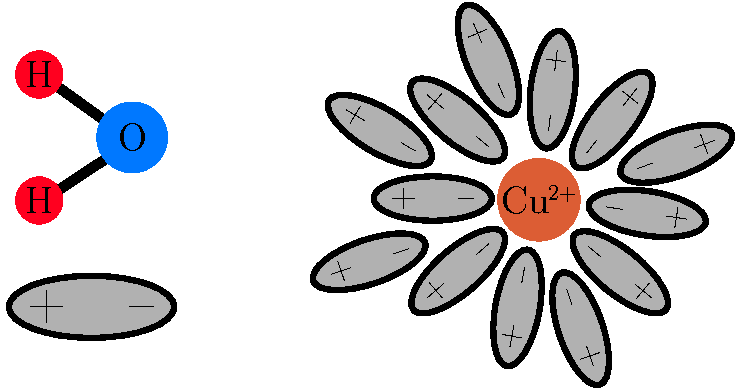
\includegraphics[width=7cm]{figs/electrolytic_dissociation/hydration.pdf}
    \caption{Вода как диполь и пример гидратации иона меди (II).}
    \label{fig:hydration}
\end{figure}

В зависимости от того, представляют собой молекулы растворителя диполь или нет, различают \textbf{полярные}\label{term:polar_solvent}\index{полярный растворитель} и \textbf{неполярные растворители}\label{term:nonpolar_solvent}\index{неполярный растворитель}.

\subsection*{Движущая сила растворимости и диссоциации}

Прежде всего нам необходимо разобраться, в чём движущая сила процессов растворимости и диссоциации. Очевидно, что для успешного протекания обоих процессов необходимо, чтобы это было выгодно энергетически. Имеются следующие вклады в суммарный эффект.

\begin{itemize}
    \item При разрыве связей между атомами в кристаллической решётке или молекуле энергия расходуется.
    \item Сольватация как ионов, так и незаряженных частиц приводит к выделению энергии.
    \item Разрыв связей между молекулами растворителя перед сольватацией приводит к поглощению энергии.
    \item Неупорядоченность системы и в процессе растворения, и в процессе диссоциации растёт.
\end{itemize}

От баланса указанных вкладов зависит, будет ли протекать растворение и диссоциация. Рассмотрим варианты взаимодействия веществ с растворителями различной полярности.

\subsection*{Неполярный растворитель и молекулярная кристаллическая решётка}

Рассмотрим энергетическую диаграмму такого взаимодействия (рис.~\ref{fig:nonpolar_solvent_and_molecular_lattice}).

\begin{figure}[htbp]
    \centering
    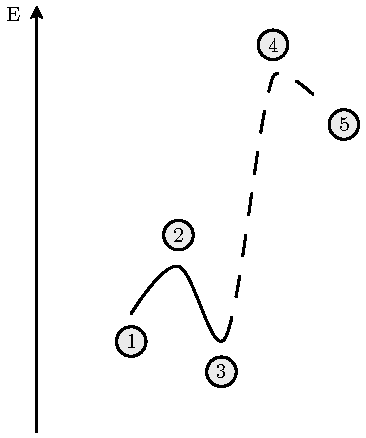
\includegraphics[width=5cm]{figs/electrolytic_dissociation/nonpolar_solvent_and_molecular_lattice.pdf}
    \caption{Неполярный растворитель и молекулярная кристаллическая решётка.}
    \label{fig:nonpolar_solvent_and_molecular_lattice}
\end{figure}

В точке \ding{172} энергетической диаграммы находятся молекулярная решётка и растворитель с межмолекулярными связями. Решётку и связи между молекулами растворителя легко разрушить, поэтому энергетический барьер \ding{173} лежит невысоко. Энергии в процессе сольватации выделяется мало, состояние растворённых сольватированных молекул \ding{174} немного выгоднее, чем исходное по энергии за счёт энтропии. Затем очень трудно разорвать ковалентные связи внутри молекулы, а энергии от сольватации ионов будет также выделяться мало (из-за неспецифической сольватации), поэтому последующая диссоциация не реализуется.

\subsection*{Неполярный растворитель и ионная кристаллическая решётка}

Ионную кристаллическую решётку невозможно сначала перевести в растворённое состояние, а затем диссоциировать, поскольку не существует отдельных молекул в ионной решётке. Оба процесса (растворение и диссоциация) протекают одновременно. Неполярный растворитель не способен специфически сольватировать ионы в растворе, поэтому как переходное состояние \ding{173}, так и продукты \ding{174} будут очень высоко по энергии. Неполярный растворитель не способен ни растворить, ни диссоциировать вещества с ионной кристаллической решёткой (рис.~\ref{fig:nonpolar_solvent_and_ionic_lattice}).

\begin{figure}[htbp]
    \centering
    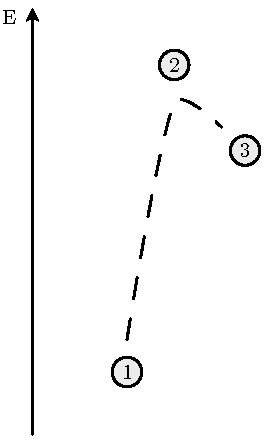
\includegraphics[width=3.7cm]{figs/electrolytic_dissociation/nonpolar_solvent_and_ionic_lattice.pdf}
    \caption{Неполярный растворитель и ионная кристаллическая решётка.}
    \label{fig:nonpolar_solvent_and_ionic_lattice}
\end{figure}

\subsection*{Полярный растворитель и молекулярная кристаллическая решётка}

Полярному растворителю сложнее разорвать связи между своими молекулами, ведь там есть как минимум взаимодействие диполей. Однако и сольватирует он более эффективно, поэтому выделившейся энергии бывает достаточно, чтобы растворить вещества с молекулярной решёткой (точка \ding{174}). Дальше процесс не происходит: растворитель может специфически сольватировать ионы, которые могли бы образоваться при диссоциации неполярных молекул, однако эти ионы лежат слишком высоко по энергии (точка \ding{175}), так как неустойчивы (рис.~\ref{fig:polar_solvent_and_molecular_lattice}).

\begin{figure}[htbp]
    \centering
    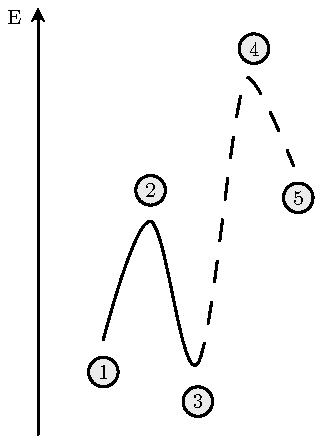
\includegraphics[width=4.5cm]{figs/electrolytic_dissociation/polar_solvent_and_molecular_lattice.pdf}
    \caption{Полярный растворитель и молекулярная кристаллическая решётка.}
    \label{fig:polar_solvent_and_molecular_lattice}
\end{figure}

\subsection*{Полярный растворитель и ионная кристаллическая решётка}

Полярный растворитель очень эффективно сольватирует ионы, точка \ding{174} лежит значительно ниже точки \ding{172}. Энергетический барьер \ding{173} преодолевается (рис.~\ref{fig:polar_solvent_and_ionic_lattice}). Подобный тип растворимости наиболее распространён.

\begin{figure}[htbp]
    \centering
    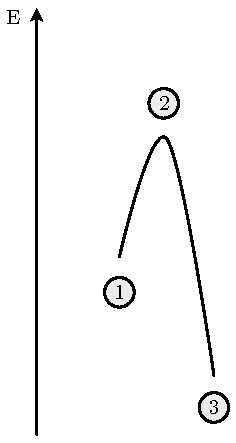
\includegraphics[width=3.5cm]{figs/electrolytic_dissociation/polar_solvent_and_ionic_lattice.pdf}
    \caption{Полярный растворитель и ионная кристаллическая решётка.}
    \label{fig:polar_solvent_and_ionic_lattice}
\end{figure}

\subsection*{Уравнения диссоциации электролитов}

Вещества, способные к электролитической диссоциации, называют \textbf{электролитами}\label{term:electrolytes}\index{электролиты}. 

Некоторые вещества полностью диссоциируют в растворителе, их называют \textbf{сильными электролитами}\label{term:strong_electrolytes}\index{сильные электролиты}. Вещества, в растворе которых не все молекулы распадаются на ионы, называют \textbf{слабыми электролитами}\label{term:weak_electrolytes}\index{слабые электролиты}. Вещества, не способные к диссоциации, называют \textbf{неэлектролитами}\label{term:nonelectrolytes}\index{неэлектролиты} (табл.~\ref{tab:examples_of_electrolytes_and_nonelectrolytes}).

\begin{table}[htbp]
    \small
    \caption{Примеры электролитов и неэлектролитов.}
    \label{tab:examples_of_electrolytes_and_nonelectrolytes}
    \begin{tabularx}{\textwidth}{
        >{\hsize=1\hsize}Z
        >{\hsize=1\hsize}Z
        }
        \hline
        \rowcolor{green!5}
        Электролиты в воде & Неэлектролиты в воде \\
        \hline
        \ce{NaBr}, \ce{KOH}, \ce{H2SO4}, \ce{Al(NO3)3} & Сахара, спирты, ацетон \\
        \hline
    \end{tabularx}
\end{table}

Для того, чтобы подчеркнуть полную диссоциацию сильных электролитов при написании уравнения диссоциации используют одностороннюю стрелку:

\reaction*{Ca(NO3)2 -> Ca^{2+} + 2NO3^-{.}}

Для слабых электролитов используют двустороннюю стрелку, подчёркивая неполную диссоциацию:

\reaction*{H2SiO3 <--> H^+ + HSiO3^-{.}}

Вещества, проявляющие свойства сильных электролитов, обычно имеют ионные или сильно полярные ковалентные связи, которые могут легко разорваться с образованием ионов.

В неэлектролитах могут присутствовать полярные, малополярные и неполярные связи, однако в этих соединениях не происходит их разрыва с образованием ионов.

Между ионом и молекулами воды зачастую образуются настолько сильные связи, что многие вещества после выпаривания растворов образуют \textbf{кристаллогидраты}\label{term:crystallohydrate}\index{кристаллогидрат}~--- соединения, содержащие некоторое количество связанных молекул воды. Часто такие соединения имеют собственные тривиальные названия, например:

\begin{itemize}
    \item \ce{CuSO4 * 5H2O}~--- медный купорос (синий);
    \item \ce{FeSO4 * 7H2O}~--- железный купорос (светло-зелёный);
    \item \ce{CaSO4 * 2H2O}~--- гипс (белый);
    \item \ce{KAl(SO4)2 * 12H2O}~--- алюмокалиевые квасцы (бесцветные);
    \item \ce{Na2SO4 * 10H2O}~--- глауберова соль (бесцветная).
\end{itemize}

Кристаллогидраты тоже образуются в случае, если выигрыш в энергии за счёт связи катиона с молекулами воды больше, чем проигрыш из-за ослабления связи с анионом в кристаллической решётке.

Многие кристаллогидраты и растворы соответствующих солей окрашены, что наглядно свидетельствует о взаимодействии ионов с молекулами воды. Как правило, окраска гидратированных ионов характерна для d-элементов, например: \ce{Co}, \ce{Cr}, \ce{Cu}, \ce{Fe}. В \hyperref[appendix:table_of_solubility_of_salts]{таблице растворимости} в приложении приведена окраска кристаллогидратов, растворов и сухих солей.

Давайте повторим новые термины и перейдём к решению задач.

\begin{termlist}
    \hyperref[term:electrolytic_dissociation]{Электролитическая диссоциация}, 
    \hyperref[term:solvation]{сольватация},
    \hyperref[term:dipole]{диполь},
    \hyperref[term:hydration]{гидратация},
    \hyperref[term:polar_solvent]{полярный растворитель},
    \hyperref[term:nonpolar_solvent]{неполярный растворитель},
    \hyperref[term:electrolytes]{электролиты},
    \hyperref[term:strong_electrolytes]{сильные электролиты},
    \hyperref[term:weak_electrolytes]{слабые электролиты},
    \hyperref[term:nonelectrolytes]{неэлектролиты},
    \hyperref[term:crystallohydrate]{кристаллогидрат}.
\end{termlist}

\begin{problem}{}{electrolytic_dissociation1}
    Почему электролиты проводят электрический ток?
    \begin{sol}{\ref{prob:electrolytic_dissociation1}}
        В них существуют заряженные частицы в растворе (ионы), способные двигаться под действием внешнего электрического поля.
    \end{sol}
\end{problem}

\begin{problem}{}{electrolytic_dissociation2}
    Как осуществить реакции:
    \reaction*{NaCl -> Na^+ + Cl^-{,}}
    \reaction*{Na^+ + Cl^- -> NaCl{,}}
    в домашних условиях?
    \begin{sol}{\ref{prob:electrolytic_dissociation2}}
        Растворением поваренной соли в воде, а затем выпариванием полученного раствора.
    \end{sol}
\end{problem}

\begin{problem}{}{electrolytic_dissociation3}
    Среди перечисленных веществ выберите электролиты: а) хлорид натрия; б) ацетон; в) сахароза; г) нитрат калия; д) серная кислота; е) бромид бария; ж) азот.
    \begin{sol}{\ref{prob:electrolytic_dissociation3}}
        а, г, д, е.
    \end{sol}
\end{problem}

\begin{problem}{}{electrolytic_dissociation4}
    Среди перечисленных веществ выберите неэлектролиты: а) борная кислота; б) аргон; в) гидроксид натрия; г) этанол; д) хлорид кальция.
    \begin{sol}{\ref{prob:electrolytic_dissociation4}}
        б, г.
    \end{sol}
\end{problem}

\begin{problem}{}{electrolytic_dissociation5}
    Что из перечисленного проводит электрический ток: а) сжиженный \ce{SO2}; б) водный раствор \ce{SO2}; в) расплав \ce{KI}; г) раствор \ce{KOH}?
    \begin{sol}{\ref{prob:electrolytic_dissociation5}}
        б, в, г. Раствор диоксида серы проводит ток из-за диссоциации образующейся при растворении сернистой кислоты:
        \reaction*{SO2 + H2O <--> H2SO3{.}}
    \end{sol}
\end{problem}

\begin{problem}{}{electrolytic_dissociation6}
    Расставьте в порядке увеличения электропроводности: а) дождевая вода; б) водопроводная вода; в) дистиллированная вода.
    \begin{sol}{\ref{prob:electrolytic_dissociation6}}
        Величина электропроводности зависит от концентрации носителей зарядов в растворе~--- диссоциирующих на ионы растворённых соединений. Дистиллированная вода самая чистая, её электропроводность будет наименьшей. Дождевая вода поглощает частички пыли и растворённые в атмосфере газы~--- \ce{CO2}, \ce{SO2}. Её электропроводность будет промежуточной. Наконец, водопроводная вода содержит значительное количество растворённых минеральных веществ и обладает наибольшей электропроводностью. Поэтому ответ: в < а < б.
    \end{sol}
\end{problem}

\clearpage

\section{Кислоты, основания и соли (теория Аррениуса)}

\textbf{Кислотами}\label{term:acid}\index{кислота} называют вещества, диссоциирующие при растворении с образованием иона водорода \ce{H^+} и \textbf{кислотного остатка}\label{term:acid_residue}\index{кислотный остаток}:

\reaction*{HCl -> H^+ + Cl^-{.}}

Растворы, в которых ионов водорода больше, чем в чистой воде, называют \textbf{кислыми}\label{term:acidic_solution}\index{кислый раствор}.

Вещества, образующие при растворении гидроксид-ионы, называют \textbf{основаниями}\label{term:base}\index{основание}:

\reaction*{NaOH -> Na^+ + OH^-{.}}

При их растворении и диссоциации в воде накапливаются гидроксид-ионы, а концентрация ионов водорода ниже, чем в чистой воде. Такие растворы называют \textbf{основными} или \textbf{щелочными}\label{term:alkaline_solution}\index{щелочной раствор}.

Вещества, диссоциирующие при растворении с образованием иных катионов (не водорода) и кислотных остатков, называются \textbf{солями}:

\reaction*{K3PO4 -> 3K^+ +PO4^{3-}{.}}

Соли, содержащие в своём составе атомы водорода, например, \ce{NaH2PO4} называются кислыми солями. Соли, содержащие в своём составе гидроксильные группы, например, \ce{(CuOH)2CO3}, называют основными солями.

\subsection*{Ступенчатая диссоциация}

Вещества, в которых полярность связей лежит в промежуточном диапазоне между ионной и ковалентной полярной, обычно диссоциируют с трудом, то есть являются слабыми электролитами. Это, например, \ce{H2S}, \ce{H3PO4}, \ce{Mg(OH)2}.

Если в них возможен отрыв сразу нескольких ионов \ce{H^+} или \ce{OH^-}, то каждая последующая стадия диссоциации энергетически всё менее выгодна из-за того, что заряд образующегося противоиона растёт:

1 ступень:

\reaction*{H3PO4 <--> H^+ + H2PO4^-{.}}

2 ступень:

\reaction*{H2PO4^- <--> H^+ + HPO4^{2-}{.}}

3 ступень (почти не происходит):

\reaction*{HPO4^{2-} <--> H^+ + PO4^{3-}{.}}

Например, гидросульфит натрия \ce{NaHSO3} имеет классическую ионную решётку и в воде полностью диссоциирует на гидросульфит-ионы и ионы натрия:

\reaction*{NaHSO3 -> Na^+ + HSO3^-{.}}

Гидросульфит-ион может диссоциировать дальше, однако это соответствует диссоциации сернистой кислоты по второй ступени, поэтому этот процесс происходит незначительно:

\reaction*{HSO3^- <--> H^+ + SO3^{2-}{.}}

\begin{termlist}
    \hyperref[term:acid]{Кислота}, 
    \hyperref[term:acid_residue]{кислотный остаток},
    \hyperref[term:acidic_solution]{кислый раствор},
    \hyperref[term:base]{основание},
    \hyperref[term:alkaline_solution]{щелочной раствор}.
\end{termlist}

\begin{problem}{}{acids_bases_and_salts1}
    Приведите примеры \emph{сильных} электролитов и напишите уравнения их электролитической диссоциации.
    \begin{sol}{\ref{prob:acids_bases_and_salts1}}
        Много вариантов, например:
        \reaction*{KI -> K^+ + I^-{,}}
        \reaction*{Al2(SO4)3 -> 2Al^{3+} + 3SO4^{2-}{.}}
    \end{sol}
\end{problem}

\begin{problem}{}{acids_bases_and_salts2}
    Приведите примеры \emph{слабых} электролитов и напишите уравнения их электролитической диссоциации.
    \begin{sol}{\ref{prob:acids_bases_and_salts2}}
        Например:
        \reaction*{H2S <--> H^+ + HS^-{,}}
        \reaction*{CH3COOH <--> H^+ + CH3COO^-{.}}
    \end{sol}
\end{problem}

\begin{problem}{}{acids_bases_and_salts3}
    В растворе имеются следующие ионы: \ce{Na^+}, \ce{Mg^{2+}}, \ce{Cl^-}, \ce{NO3^-}. Какие соли могли быть взяты для получения этого раствора?
    \begin{sol}{\ref{prob:acids_bases_and_salts3}}
        \ce{NaCl + Mg(NO3)2} или \ce{NaNO3 + MgCl2}.
    \end{sol}
\end{problem}

\begin{problem}{}{acids_bases_and_salts4}
    Предложите способ обнаружения присутствия растворимых солей в образце почвы.
    \begin{sol}{\ref{prob:acids_bases_and_salts4}}
        Образец почвы промывается дистиллированной водой, промывная вода затем проверяется на электропроводность.
    \end{sol}
\end{problem}

\begin{problem}{}{acids_bases_and_salts5}
    Напишите уравнения электролитической диссоциации следующих соединений:
    \begin{enumerate}[label=\arabic*)]
        \item \ce{HCl};
        \item \ce{Sr(NO3)2};
        \item \ce{H2SiO3}.
    \end{enumerate}
    \begin{sol}{\ref{prob:acids_bases_and_salts5}}
        \begin{enumerate}[label=\arabic*)]
            \item \ce{HCl -> H^+ + Cl^-};
            \item \ce{Sr(NO3)2 -> Sr^{2+} + 2NO3^-};
            \item \ce{H2SiO3 <--> H^+ + HSiO3^-}.
        \end{enumerate}
    \end{sol}
\end{problem}

\begin{problem}{}{acids_bases_and_salts6}
    Напишите уравнения электролитической диссоциации следующих соединений: 
    \begin{enumerate}[label=\arabic*)]
        \item \ce{KAl(SO4)2};
        \item \ce{Zn(OH)Cl};
        \item \ce{NaHS}.
    \end{enumerate}
    \begin{sol}{\ref{prob:acids_bases_and_salts6}}
        \begin{enumerate}[label=\arabic*)]
            \item \ce{KAl(SO4)2 -> K^+ + Al^{3+} + 2SO4^{2-}};
            \item \ce{Zn(OH)Cl -> Zn(OH)^+ + Cl^-};
            \item \ce{NaHS -> Na^+ + HS^-}.
        \end{enumerate}
        Диссоциация по второй ступени происходит крайне незначительно.
    \end{sol}
\end{problem}

\begin{problem}{}{acids_bases_and_salts7}
    Среди перечисленных ниже соединений выберите электролиты, диссоциирующие ступенчато: а) \ce{H2S}; б) \ce{H3PO4}; в) \ce{Na2SO4}; г) \ce{KHSO4}; д) \ce{NiCl2}.
    \begin{sol}{\ref{prob:acids_bases_and_salts7}}
        а, б, г.
    \end{sol}
\end{problem}

\begin{problem}{}{acids_bases_and_salts8}
    В литре воды растворили \qty{1}{\mole} хлорида магния и \qty{1}{\mole} нитрата лития. Предложите другой вариант смеси солей (включая исходные вещества), которые могли быть взяты для получения точно такого же раствора.
    \begin{sol}{\ref{prob:acids_bases_and_salts8}}
        Определяем количества веществ ионов в образовавшемся растворе согласно уравнениям диссоциации:
        \reaction*{MgCl2 -> Mg^{2+} + 2Cl^-{,}}
        \reaction*{LiNO3 -> Li^+ + NO3^-{.}}
        При растворении \qty{1}{\mole} хлорида магния в растворе оказалось \qty{1}{\mole} ионов магния и \qty{2}{\mole} хлорид-ионов. При растворении \qty{1}{\mole} нитрата лития в растворе оказалось \qty{1}{\mole} ионов лития и \qty{1}{\mole} нитрат-анионов.
        \begin{itemize}
            \item \ce{Mg^{2+}}~--- \qty{1}{\mole};
            \item \ce{Cl^-}~--- \qty{2}{\mole};
            \item \ce{Li^+}~--- \qty{1}{\mole};
            \item \ce{NO3^-}~--- \qty{1}{\mole}.
        \end{itemize}
        Если взять для приготовления раствора нитрат магния, то его количество не может превышать \qty{0,5}{\mole}, поскольку общая концентрация нитрат-анионов не может превышать \qty{1}{\mole}. Оставшееся количество магния необходимо внести в виде хлорида магния, а оставшееся количество хлорид-ионов нужно внести в виде хлорида лития:
        \begin{itemize}
            \item \ce{Mg(NO3)2}~--- \qty{0,5}{\mole};
            \item \ce{MgCl2}~--- \qty{0,5}{\mole};
            \item \ce{LiCl}~--- \qty{1}{\mole}.
        \end{itemize}
    \end{sol}
\end{problem}

\begin{problem}{}{acids_bases_and_salts9}
    Заполните пропуски в таблице <<формулы и заряды ионов в составе солей>> (K~--- катион, A~--- анион):
    \begin{table}[H]
    \small
    \begin{tabularx}{\textwidth}{
        >{\hsize=1\hsize}Z
        >{\hsize=1\hsize}Z
        >{\hsize=1\hsize}Z
        }
        \hline
        \rowcolor{green!5}
        Заряд катиона & Заряд аниона & Формула соли \\
        \hline
        ? & ? & \ce{K3A} \\
        \hline
        $+2$ & $-3$ & ? \\
        \hline
        $+1$ & ? & \ce{KA} \\
        \hline
        ? & $-1$ & \ce{KA3} \\
        \hline
        $+1$ & ? & \ce{K_?A2} \\
        \hline
    \end{tabularx}
    \end{table}
    \begin{sol}{\ref{prob:acids_bases_and_salts9}}
        Заполненная таблица:
        \begin{table}[H]
        \small
        \begin{tabularx}{\textwidth}{
            >{\hsize=1\hsize}Z
            >{\hsize=1\hsize}Z
            >{\hsize=1\hsize}Z
            }
            \hline
            \rowcolor{green!5}
            Заряд катиона & Заряд аниона & Формула соли \\
            \hline
            $+1$ & $-3$ & \ce{K3A} \\
            \hline
            $+2$ & $-3$ & \ce{K3A2} \\
            \hline
            $+1$ & $-1$ & \ce{KA} \\
            \hline
            $+3$ & $-1$ & \ce{KA3} \\
            \hline
            $+1$ & $-1$ & \ce{K2A2} \\
            \hline
        \end{tabularx}
        \end{table}
        В реальности соль с формулой \ce{K2A2} записывалась бы как \ce{KA}.
    \end{sol}
\end{problem}

\begin{problem}{}{acids_bases_and_salts10}
    Рассмотрите установку для изучения движения окрашенных ионов в электрическом поле:
    \begin{figure}[H]
        \centering
        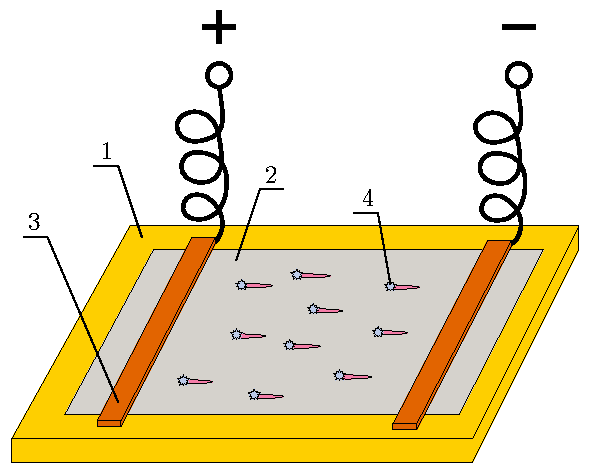
\includegraphics[width=7cm]{figs/acids_bases_and_salts/colored_ions_movement.pdf}
    \end{figure}
    На основание \ding{172} помещена пропитанная раствором неокрашенного электролита бумага \ding{173}, концы которой прижаты электродами \ding{174}. На бумагу помещают кристаллы исследуемых солей \ding{175}, которые частично растворяются в электролите. Находящиеся ионы начинают двигаться к соответствующему электроду, при этом на бумаге образуется окрашенный <<хвост>> цвета соответствующего иона. Ответьте на следующие вопросы:
    \begin{enumerate}[label=\arabic*)]
        \item Какой знак заряда имеет катод и какой анод?
        \item Как доказать, какой знак заряда имеют окрашенные ионы?
        \item В сторону катода или анода будет наблюдаться окрашенный <<хвост>> в случае исследования перманганата калия?
        \item При исследовании неизвестного вещества выяснилось, что <<хвост>> в направлении катода имеет слабо-розовое окрашивание. Пользуясь \hyperref[appendix:table_of_solubility_of_salts]{второй частью таблицы растворимости} из приложения, определите, какой ион находится в составе соли.
    \end{enumerate}
    \begin{sol}{\ref{prob:acids_bases_and_salts10}}
        Ответы на вопросы:
        \begin{enumerate}[label=\arabic*)]
            \item Катод имеет знак заряда минус $(-)$, а анод плюс $(+)$. Простое мнемоническое правило, позволяющее запомнить знаки: в парах слов <<катод>> и <<минус>>, <<анод>> и <<плюс>> по одинаковому числу букв в каждом слове.
            \item Чтобы доказать знак заряда окрашенного иона нужно определить к какому электроду он движется: если к катоду, то ион положительно заряжен, если к аноду~--- то отрицательно.
            \item В сторону анода.
            \item \ce{Co^{2+}}.
        \end{enumerate}
    \end{sol}
\end{problem}

\begin{problem}{}{acids_bases_and_salts11}
    Приведите электронные конфигурации следующих ионов: а) \ce{Li^+}; б) \ce{H^+}; в) \ce{F^-}; г) \ce{Cl^-}.
    \begin{sol}{\ref{prob:acids_bases_and_salts11}}
        а) [He]; б) $1\text{s}^0$; в) [Ne]; г) [Ar].
    \end{sol}
\end{problem}

\begin{problem}{}{acids_bases_and_salts12}
    $\bigstar$ К раствору медного купороса голубого цвета прилили концентрированный раствор хлорида натрия. При этом цвет раствора изменился на зелёный. Почему?
    \begin{sol}{\ref{prob:acids_bases_and_salts12}}
        Появление большого количества хлорид-ионов в растворе приводит к тому, что голубой гидратированный ион \ce{[Cu(H2O)6]^{2+}} превращается в жёлто-зелёный комплексный ион \ce{[CuCl4]^{2-}}. Смесь голубого и жёлтого даёт зелёный цвет.
    \end{sol}
\end{problem}

\begin{problem}{}{acids_bases_and_salts13}
    $\bigstar$ Концентрированные растворы хлорида кобальта \ce{CoCl2} имеют фиолетовый цвет. Разбавленные растворы этой же соли имеют розовый цвет.
    \begin{enumerate}[label=\arabic*)]
        \item Какова окраска гидратированных ионов \ce{Co^{2+}}?
        \item Какова окраска комплексного иона, образующегося в концентрированных растворах?
    \end{enumerate}
    \begin{sol}{\ref{prob:acids_bases_and_salts13}}
        Цвет гидратированного катиона соответствует цвету разбавленного раствора, поэтому окраска гидратированных ионов \ce{[Co(H2O)6]^{2+}}~--- розовая. Поскольку при концентрировании раствора окраска становится фиолетовой, значит в растворе возникают комплексные ионы \ce{[CoCl4]^{2-}}, цвет которых смешивается с розовым цветом. Цвет, который при смешении с розовым даёт фиолетовый цвет~--- синий или голубой. Поэтому окраска ионов \ce{[CoCl4]^{2-}} должна быть соответствующей.
    \end{sol}
\end{problem}

\clearpage

\section{Ионное произведение воды. Водородный показатель}

Измерения показывают, что чистая вода очень плохо, но всё же проводит электрический ток. Это происходит потому, что вода \emph{сама является электролитом}, то есть диссоциирует на ионы:

\reaction*{H2O <--> H^+ + OH^-{.}}

В воде и водных растворах веществ устанавливается равновесие между содержанием ионов водорода и гидроксид-ионов. Это соотношение представляет собой константу при фиксированной температуре. Эта константа равна:

\begin{equation*}
    K' = \frac{[\ce{H^+}][\ce{OH^-}]}{[\ce{H2O}]}.
\end{equation*}

Измерения показали, что значение этой константы при \qty{25}{\degreeCelsius} равно \num{1,8e-16}, то есть диссоциирует очень незначительное количество молекул воды.

Учитывая, что количество продиссоциировавших молекул почти не влияет на концентрацию исходных молекул воды, концентрацию $[\ce{H2O}]$ можно считать постоянной величиной. Рассчитаем её, взяв за образец \qty{1}{\kg} воды:

\begin{equation*}
    c_{\ce{H2O}} = \frac{m}{MV} = \frac{\qty{1000}{\g}}{\qty{18}{\g\per\mole} \cdot \qty{1}{\l}} = \qty{55,56}{\mole\per\l}.
\end{equation*}

Внесём концентрацию $[\ce{H2O}]$ в значение константы диссоциации, домножив обе части уравнения на $[\ce{H2O}]$. Мы получим другую константу, которую обозначим $K_w$:

\begin{equation*}
    K'[\ce{H2O}] = \fbox{$[\ce{H^+}][\ce{OH^-}] = K_w$}.
\end{equation*}

Величина $K_w = K'[\ce{H2O}] = \num{1,8e-16} \cdot \num{55,56} = \qty{e-14}{\mole\squared\per\l\squared}$ называется \textbf{ионным произведением воды}\label{term:ionic_product_of_water}\index{ионное произведение воды} или \textbf{константой автопротолиза}. Слово <<автопротолиз>> означает, что вода протонирует сама себя. Это выражение показывает, что в воде при данной температуре произведение молярных концентраций протонов и гидроксид-ионов является постоянной величиной, то есть при уменьшении концентрации одних будет расти концентрация других.

\subsection*{Водородный показатель}

Для того чтобы количественно охарактеризовать кислотные или осн\'{о}вные свойства растворов необходимо знать в них концентрацию ионов водорода (или гидроксид-ионов, поскольку их концентрации связаны через ионное произведение).

В химии в качестве стандартной меры кислотности или основности растворов принято использовать концентрацию ионов водорода с использованием так называемого водородного показателя.

\textbf{Водородный показатель}\label{term:pH}\index{водородный показатель} обозначается pH и равен десятичному логарифму молярной концентрации ионов водорода в растворе (выраженной в \unit{\mole\per\l}), взятому с обратным знаком:

\begin{equation*}
    \fbox{$\text{pH} = -\lg[\ce{H^+}]$}. 
\end{equation*}

Обратное вычисление концентрации ионов водорода при известном pH производится исходя из определения логарифма:

\begin{equation*}
    \fbox{$[\ce{H^+}] = 10^{-\text{pH}}$}.
\end{equation*}

Используют также совершенно аналогичную единицу для измерения концентрации гидроксид-ионов в растворе~--- pOH:

\begin{equation*}
    \text{pOH} = -\lg[\ce{OH^-}].
\end{equation*}

Термин <<водородный показатель>> был введён в 1909 году датским химиком Сёреном Сёренсеном. По одной из версий, буква <<p>> является первой буквой латинского слова <<\textit{potens}>>~--- математическая степень, H~--- символ водорода.

Рассчитаем pH чистой воды. В соответствии с уравнением диссоциации воды при автопротолизе образуется равное количество ионов водорода и гидроксид-ионов, поэтому

\begin{equation*}
    K_w = [\ce{H^+}][\ce{OH^-}] = [\ce{H^+}]^2,
\end{equation*}

отсюда

\begin{equation*}
    [\ce{H^+}] = \sqrt{K_w} = \sqrt{\num{e-14}} = \qty{e-7}{\mole\per\l},
\end{equation*}
\begin{equation*}
    \text{pH} = -\lg\num{e-7} = 7.
\end{equation*}

Таким образом, pH чистой воды при \qty{25}{\degreeCelsius} равен 7. Раствор с таким значением pH называют \textbf{нейтральным}\label{term:neutral_solution_pH}\index{нейтральный раствор (pH)}. Если $\text{pH} < 7$, то концентрация ионов водорода в таком растворе становится выше \qty{e-7}{\M}, а концентрация гидроксид-ионов снижается ниже \qty{e-7}{\M}. Такой раствор называют \textbf{кислым}\label{term:acidic_solution_pH}\index{кислый раствор (pH)}. В противном случае говорят о \textbf{щелочном}\label{term:alkaline_solution_pH}\index{щелочной раствор (pH)} растворе (рис.~\ref{fig:pH_scale}).

\begin{figure}[htbp]
    \centering
    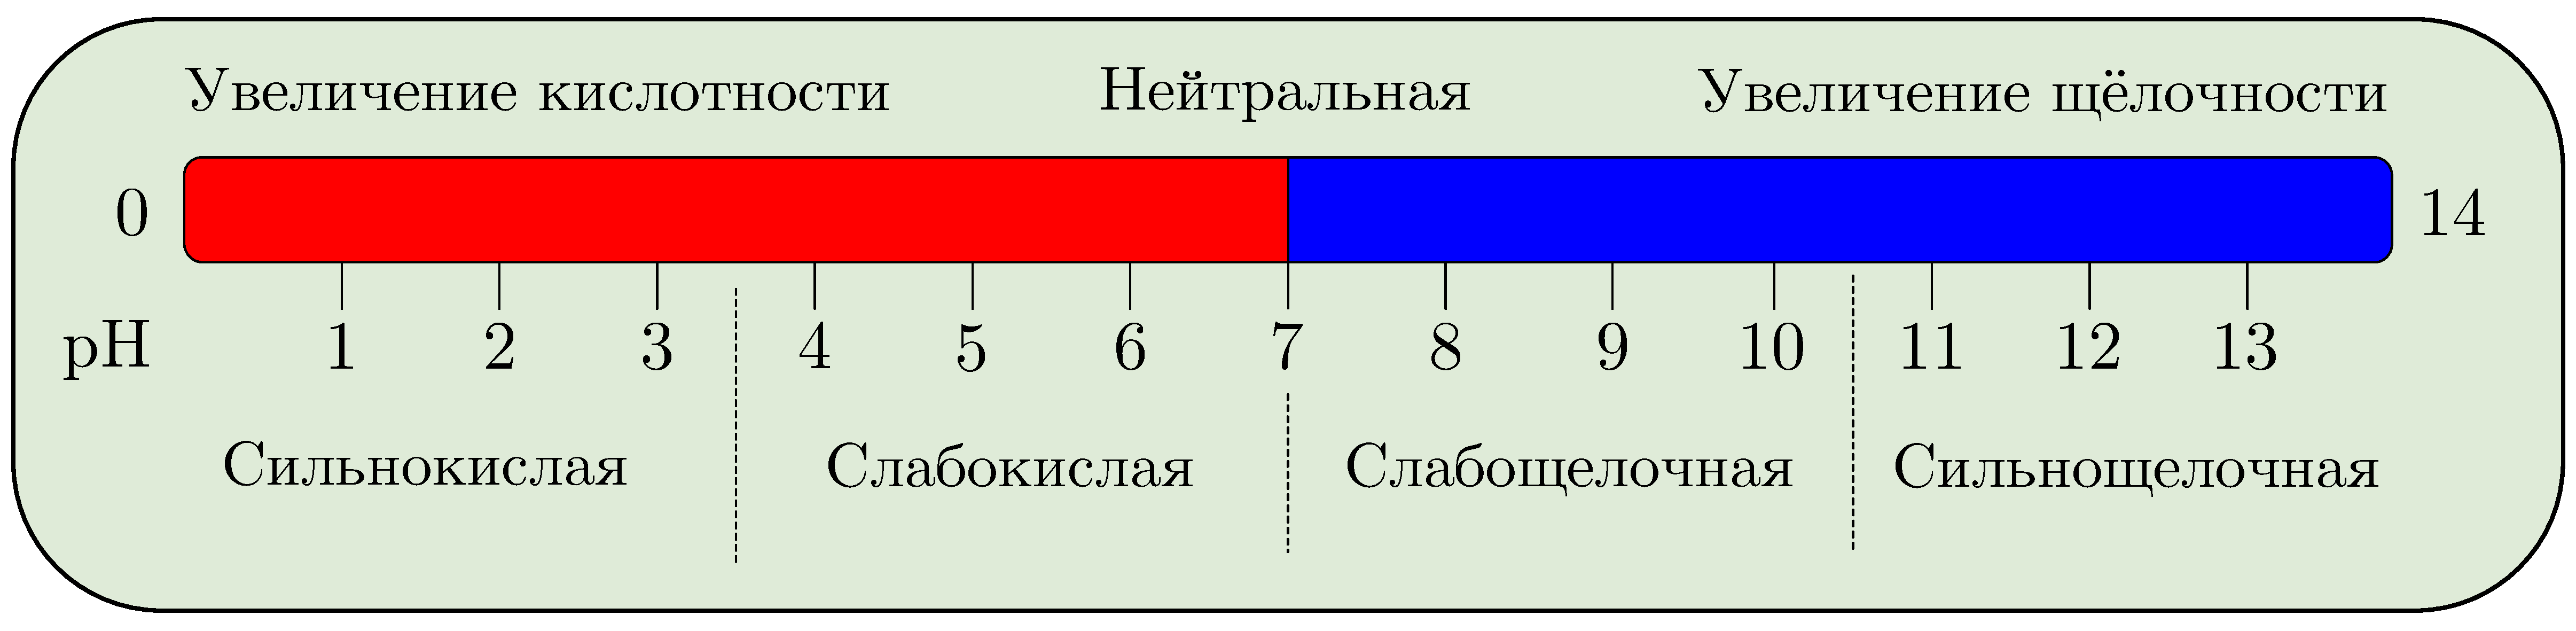
\includegraphics[width=13cm]{figs/pH/pH_scale.pdf}
    \caption{Шкала pH.}
    \label{fig:pH_scale}
\end{figure}

Диапазон pH от 0 до 14 является условным и подходит для большинства водных растворов. Однако в некоторых случаях pH может быть меньше нуля или больше 14.

\subsection*{Кислотно-основные индикаторы}

Существуют вещества, которые имеют различную окраску при различных значениях pH раствора. Такие вещества называются \textbf{кислотно-осн\'{о}вными индикаторами}\label{term:acid_base_indicator}\index{кислотно-основный индикатор}. Обычно они используются для определения среды и изменения pH невооружённым глазом, например, при титровании. Например, три известных индикатора: метиловый оранжевый, лакмус\footnote{Лакмус вошёл в употребление около 1300 года н.э., его связывают с испанским алхимиком и врачом Арнольдусом де Вилла Нова. Современное слово <<\textit{litmus}>> происходит от древнескандинавского слова, означающего <<краска>> или <<цвет>>.} и фенолфталеин\footnote{При высоких pH (>13) фенолфталеин снова становится бесцветным, то есть меняет окраску дважды.} (табл.~\ref{tab:pH_indicator_colors}). В приложении~\ref{appendix:pH_indicator_colors} представлены и другие распространённые индикаторы.

\begin{table}[htbp]
    \small
    \caption{Цвета распространённых кислотно-основных индикаторов.}
    \label{tab:pH_indicator_colors}
    \begin{tabularx}{\textwidth}{
        >{\hsize=1.6\hsize}Y
        >{\hsize=0.8\hsize}Z
        >{\hsize=0.8\hsize}Z
        >{\hsize=0.8\hsize}Z
        }
        \hline
        \rowcolor{green!5}
        Название индикатора & Цвет в более кислой области & Интервал перехода & Цвет в более щелочной области \\
        \hline
        Метиловый оранжевый & \cellcolor{methyl_orange_acid} & \num{3,1}--\num{4,4} & \cellcolor{methyl_orange_base} \\
        \hline
        Лакмус & \cellcolor{litmus_acid} & \num{5,0}--\num{8,0} & \cellcolor{litmus_base} \\
        \hline
        Фенолфталеин & бесцветный & \num{8,2}--\num{10,0} & \cellcolor{phenolphthalein_base} \\
        \hline
    \end{tabularx}
\end{table}

Переход окраски происходит не мгновенно, а плавно, в определённом диапазоне pH, который называется \textbf{интервалом перехода}\label{term:color_change_interval}\index{интервал перехода}, при этом цвет меняется постепенно, поэтому по окраске индикатора можно судить лишь о том, \emph{в каком интервале} находится pH раствора в данный момент.

\begin{termlist}
    \hyperref[term:ionic_product_of_water]{Ионное произведение воды}, 
    \hyperref[term:pH]{водородный показатель},
    \hyperref[term:neutral_solution_pH]{нейтральный раствор},
    \hyperref[term:acidic_solution_pH]{кислый раствор},
    \hyperref[term:alkaline_solution_pH]{щелочной раствор},
    \hyperref[term:acid_base_indicator]{кислотно-основный индикатор},
    \hyperref[term:color_change_interval]{интервал перехода}.
\end{termlist}

\begin{problem}{}{pH1}
    Известно, что ионное произведение воды растёт с повышением температуры. Экзотермической или эндотермической является реакция диссоциации воды?
    \begin{sol}{\ref{prob:pH1}}
        Поскольку повышение температуры приводит к увеличению диссоциации (равновесие смещено в сторону продуктов реакции), то в соответствии с принципом Ле Шателье реакция является эндотермической (происходит с поглощением тепла).
    \end{sol}
\end{problem}

\begin{problem}{}{pH2}
    Вычислите pH раствора, в котором концентрация ионов водорода равна \qty{e-3}{\M}.
    \begin{sol}{\ref{prob:pH2}}
        3.
    \end{sol}
\end{problem}

\begin{problem}{}{pH3}
    Вычислите pOH раствора, в котором концентрация гидроксид ионов равна \qty{e-4}{\M}.
    \begin{sol}{\ref{prob:pH3}}
        4.
    \end{sol}
\end{problem}

\begin{problem}{}{pH4}
    Пользуясь выражением ионного произведения воды, вычислите, чему равна сумма pH + pOH любого водного раствора.
    \begin{sol}{\ref{prob:pH4}}
        Прологарифмируем ионное произведение воды:
        \begin{equation*}
            \lg{K_w} = \lg([\ce{H^+}][\ce{OH^-}]) = \lg[\ce{H^+}] + \lg[\ce{OH^-}],
        \end{equation*}
        \begin{equation*}
            -\lg{K_w} = -\lg[\ce{H^+}] - \lg[\ce{OH^-}],
        \end{equation*}
        \begin{equation*}
            \text{pH} + \text{pOH} = -\lg{K_w} = -\lg 10^{-14} = 14.
        \end{equation*}
    \end{sol}
\end{problem}

\begin{problem}{}{pH5}
    Вычислите двумя способами pH раствора, содержащего \qty{e-5}{\M} гидроксид-ионов.
    \begin{sol}{\ref{prob:pH5}}
        Первый способ:
        \begin{equation*}
            [\ce{H^+}] = \frac{K_w}{[\ce{OH^-}]} = \frac{10^{-14}}{10^{-5}} = \qty{e-9}{\M},
        \end{equation*}
        \begin{equation*}
            \text{pH} = -\lg[\ce{H^+}] = -\lg{10^{-9}} = 9.
        \end{equation*}
        Второй способ:
        \begin{equation*}
            \text{pOH} = -\lg[\ce{OH^-}] = -\lg{10^{-5}} = 5,
        \end{equation*}
        \begin{equation*}
            \text{pH} = 14 - \text{pOH} = 14 - 5 = 9.
        \end{equation*}
    \end{sol}
\end{problem}

\begin{problem}{}{pH6}
    pH лимонного сока примерно равен \num{2,1}. Чему равна концентрация ионов водорода в нём?
    \begin{sol}{\ref{prob:pH6}}
        Воспользуемся определением водородного показателя:
        \begin{equation*}
            [\ce{H^+}] = 10^{-\text{pH}} = 10^{-2,1} = \qty{7,94e-3}{\M}.
        \end{equation*}
    \end{sol}
\end{problem}

\begin{problem}{}{pH7}
    pH вина составляет примерно \num{3,5}. Чему равно соотношение ионов водорода и гидроксид-ионов в нём?
    \begin{sol}{\ref{prob:pH7}}
        \textit{1 способ (постадийный)}. Вычислим концентрацию ионов водорода:
        \begin{equation*}
            [\ce{H^+}] = 10^{-\text{pH}} = 10^{-3,5} = \qty{3,16e-4}{\M}.
        \end{equation*}
        Концентрацию гидроксид-ионов найдём из ионного произведения воды:
        \begin{equation*}
            [\ce{OH^-}] = \frac{K_w}{[\ce{H^+}]} = \frac{10^{-14}}{\num{3,16e-4}} = \qty{3,16e-11}{\M}.
        \end{equation*}
        Соотношение ионов водорода и гидроксид-ионов будет равно:
        \begin{equation*}
            \frac{[\ce{H^+}]}{[\ce{OH^-}]} = \frac{\num{3,16e-4}}{\num{3,16e-11}} = 10^7.
        \end{equation*}
        \textit{2 способ (формульный)}. Можно не считать концентрации по стадиям, а сразу вывести итоговую формулу:
        \begin{equation*}
            \frac{[\ce{H^+}]}{[\ce{OH^-}]} = \frac{10^{-\text{pH}} \cdot 10^{-\text{pH}}}{K_w} = \frac{10^{-2\text{pH}}}{K_w} = \frac{10^{-2 \cdot \num{3,5}}}{10^{-14}} = 10^7.
        \end{equation*}
        Таким образом, в вине на один гидроксид-ион приходится десять миллионов ионов водорода.
    \end{sol}
\end{problem}

\begin{problem}{}{pH8}
    Как вы считаете, почему для величины pH используют именно десятичный логарифм, а не какой-нибудь другой, например, натуральный?
    \begin{sol}{\ref{prob:pH8}}
        Это связано с тем, что мы используем десятичную систему счисления и десятичный логарифм наиболее удобен, поскольку мы сразу можем оценить его значение по величине степени в научной записи числа, например, $\lg10^8 = 8$.
    \end{sol}
\end{problem}

\begin{problem}{}{pH9}
    $\bigstar$ В некоторой параллельной вселенной ионное произведение воды равно \num{e-10}. Ответьте на некоторые вопросы:
    \begin{enumerate}[label=\arabic*)]
        \item Чему равен pH чистой воды в этой вселенной?
        \item Какую реакцию среды (кислую или щелочную) имеет в этой вселенной раствор с $\text{pH} = 6$?
        \item Вычислите, чему равна в этой вселенной сумма $\text{pH} + \text{pOH}$.
    \end{enumerate}
    \begin{sol}{\ref{prob:pH9}}
        \begin{enumerate}[label=\arabic*)]
            \item $\text{pH} = -\lg\sqrt{K_w} = -\lg(10^{-5}) = 5$.
            \item Щелочную.
            \item $\text{pH} + \text{pOH} = -\lg{K_w} = -\lg{10^{-10}} = 10$.
        \end{enumerate}
    \end{sol}
\end{problem}

\begin{problem}{}{pH10}
    $\bigstar$ Для приготовления смешанного индикатора смешали фенолфталеин и лакмус. Какое окрашивание будет наблюдаться при $\text{pH} = 3$? $\text{pH} = 12$?
    \begin{sol}{\ref{prob:pH10}}
       В кислом растворе будет окрашен только лакмус: цвет раствора будет красный. В щелочном растворе будут окрашены оба индикатора: цвет раствора будет образован смешиванием двух индикаторных цветов~--- синего и малинового, поэтому будет наблюдаться фиолетовое окрашивание.
    \end{sol}
\end{problem}

\clearpage

\section{\# Кислотность почвы}

Химия, как и любая естественная наука, сочетает в себе как фундаментальную, так и прикладную составляющие, отражая практическую пользу образования, которую можно сформулировать в виде известного тезиса <<знание --- сила>>.

Рассмотренный нами водородный показатель используется в науке буквально везде как общий индикатор кислотности. Давайте рассмотрим его применение в одном из практических аспектов, в частности, для характеристики кислотности почвы и как им пользоваться при выращивании растений.

\subsection*{Что такое почва}

\begin{wrapfigure}{r}{0.35\textwidth}
    \centering
    
\includegraphics[width=4cm]{figs/soil_acidity/soil.pdf}
\end{wrapfigure}

Вы, разумеется, замечали, что в определённых местах в вашей местности предпочитают произрастать отдельные группы растений. Например, можжевельник всегда соседствует с соснами, клюква растёт на болоте, папоротники и ландыши часто оказываются по соседству, а капуста, свекла и морковь на торфяниках дают крайне низкий урожай. Разумеется, причина этого в том, что различным растениям необходимы подходящие условия для их нормального развития.

Таких условий много: это общий климат местности, увлажнённость почвы, соседство с другими растениями и наличие питательных веществ, в том числе и минеральный состав почвы.

\textbf{Почва}~--- это верхний плодородный слой земной коры, состоящий из сложной смеси органических и неорганических веществ. Она образуется в результате действия биосферы на верхний слой горных пород. Она содержит, кроме непосредственно частиц породы, на которой образуется, отмершую органику, минеральные соли, простые органические соединения, части живых организмов, растущие в ней в данный момент, а также части животного происхождения (организмы, населяющие почву, и продукты их жизнедеятельности).

Растения, произрастающие на слое почвы, используют её как субстрат для удержания при помощи корневой системы и извлекают из неё минеральные вещества (для растений в первую очередь важны азот, фосфор и калий) и микроэлементы, которые потом возвращаются обратно в почву при отмирании растений и животных. При этом содержание полезных веществ и способность растений расти сильно зависит от \emph{кислотности} (pH) почвы.

\subsection*{Почва как химическая модель}

Чтобы понять закономерности изменения кислотности почвы, представим почву в виде двухфазной системы: матрица из твёрдых частиц различного размера и водный раствор, распределённый между частицами. В этой системе твёрдые частицы, составляющие почву, способны обмениваться ионами и молекулами веществ с водной фазой.

Между твёрдой и жидкой фазами почвы устанавливается равновесие по концентрациям веществ, поэтому выводы о почве нельзя сделать только на основе состава жидкой фазы.

Твёрдая фаза почвы, способная поглощать и обменивать поглощенные ионы, называется \textbf{почвенным поглощающим комплексом} (ППК). Его состав чрезвычайно сложен. ППК состоит в первую очередь из неорганических минералов, содержащих алюмосиликаты, карбонаты и оксиды кальция, марганца и железа, и органических веществ сложного состава, образованных перегнившей органикой (рис.~\ref{fig:soil_absorption_complex}).

\begin{figure}[htbp]
    \centering
    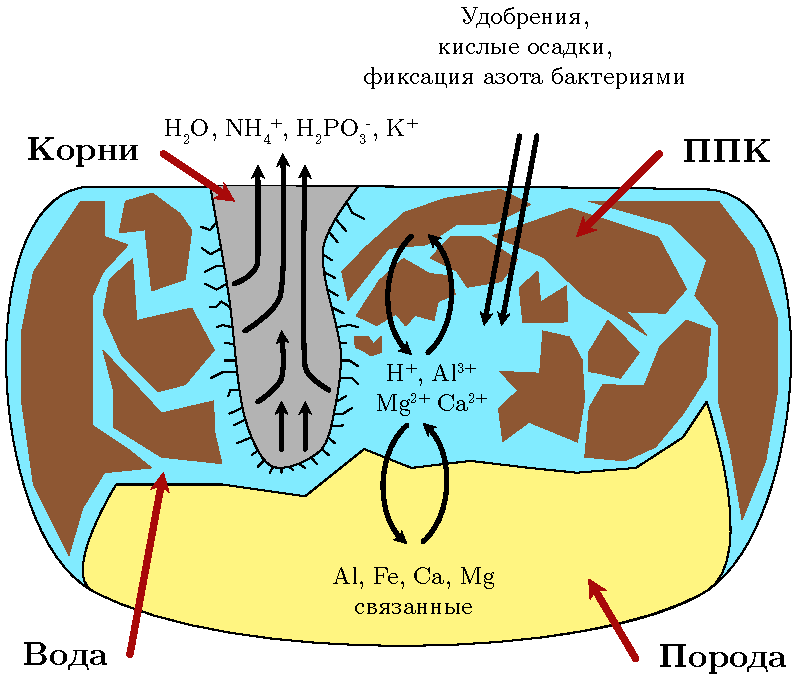
\includegraphics[width=10cm]{figs/soil_acidity/soil_absorption_complex.pdf}
    \caption{Устройство почвенного поглощающего комплекса.}
    \label{fig:soil_absorption_complex}
\end{figure}

Растения взаимодействуют в первую очередь с жидкой фазой почвы, которая затем меняет свой состав в ходе процессов обмена веществом с ППК.  Другими словами, существует <<явная>> кислотность, определяющаяся концентрацией \ce{H+} в водной фазе в данный момент и <<скрытая>>, которая может быть извлечена (или поглощена!) из ППК.

Фактически, ППК проявляет свойства буферных систем, которые мы будем изучать далее, но пока для понимания работы почвенного комплекса можно обойтись тем, что твёрдая фаза почвы способна принимать или отдавать протоны и другие вещества в зависимости от создаваемых условий.

Давайте сформулируем факторы, определяющие кислотность почвы:

\begin{itemize}
    \item минеральный состав исходной породы, на которой формируется почва;
    \item как двигается вода в почве: промывая ППК в сторону породы или поднимаясь по капиллярам из породы в ППК;
    \item диссоциация органических кислот из отмершей органики и количество этой органики;
    \item внесение веществ человеком (удобрения, кислотные дожди и пр.).
\end{itemize}

\subsection*{Как измерить кислотность почвы}

Существует несколько показателей кислотности почвы в зависимости от того, чем она обусловлена и как изменяется при воздействии на неё различных веществ.

Очевидно, что мы в первую очередь можем измерить кислотность водной фазы почвы. Этот показатель называется \textbf{активной кислотностью}~--- это pH почвенной вытяжки, полученной при промывке почвы водой. Поскольку значительная часть кислотности <<спрятана>> в ППК, активной кислотности недостаточно.

\textbf{Обменная кислотность} определяется при обработке пробы почвы \ce{KCl}. Ионы \ce{K+} вытесняют \ce{H+} и \ce{Al^{3+}} из ППК в раствор, она показывает, как почва будет себя вести при внесении удобрений.

\textbf{Гидролитическая кислотность} или \textbf{полная кислотность}~--- определяется гидролитически щелочным раствором \ce{CH3COONa}. По сути, это максимальная доза щелочных веществ, которые способна поглотить почва, именно она используется для расчёта доз известняка для раскисления почвы (об этом расскажем ниже).

Попробуйте определить активную кислотность интересующей вас почвы, поскольку технически это сделать проще всего.

Чтобы понять, какова кислотность почвы на вашем участке, нельзя просто взять землю из понравившегося места и приложить к ней индикаторную бумагу. Для измерения кислотности необходимо правильно провести отбор проб и пробоподготовку, чтобы обеспечить репрезентативность выборки\footnote{То есть гарантировать, что отобранная проба действительно характеризует почву на всём участке, а не на отдельных его частях. Неправильный отбор проб приводит к нерепрезентативной выборке и, как следствие, неверным результатам. К примеру, типичными ошибками являются взятие проб почвы только с одной точки участка или только с поверхности.}.

Итак, на том участке, где необходимо оценить кислотность почвы, нужно отобрать примерно по \qty{50}{\g} почвы с поверхности и из глубины \qty{10}{\cm} из точек на краях участка и из его середины. Смешайте все пробы и выложите смесь на подходящую поверхность, дождавшись, пока почва не высохнет. Раздавите все крупные куски почвы больше горошины до состояния порошка. Перемешайте образец и разровняйте его на подходящей поверхности в виде круга.

Полученный круг разделите на четыре равных сектора, землю из первого и третьего секторов выбросьте, а из второго и четвёртого смешайте вместе и выложите новый круг. Повторите эту операцию до тех пор, пока не останется примерно \qty{25}{\g} почвы\footnote{Эта операция называется \textbf{квартование}, её смысл в том, чтобы обеспечить равномерное смешивание вещества пробы.}.

К полученной пробе добавьте \qty{75}{\g} холодной дистиллированной воды и тщательно перемешайте полученную суспензию в течение нескольких минут. Затем дайте отстояться пробе, пока жидкость не станет светлой, и измерьте pH жидкости универсальной индикаторной бумагой.

В зависимости от полученного pH почва окажется \textbf{кислой} (pH < 7) или \textbf{щелочной} (pH > 7). Также кислотность почвы может оказаться близкой к \textbf{нейтральной} (примерно равна 7).

Измеренное значение активной кислотности не будет полностью характеризовать почву, но вполне подойдёт для первичной оценки. Тем не менее помните, что при измерении активной кислотности вы можете получить нейтральное значение, а почва на самом деле будет сильно кислой и нуждаться в известковании. Поэтому в профессиональных агрохимических лабораториях почти никогда не используют простую водную вытяжку для анализа и рекомендаций. Правильный выход из данной ситуации: используйте полученное значение активной кислотности совместно с наличием растений-индикаторов для общего вывода о кислотности почвы либо, если есть доступ к лаборатории – проведите измерение гидролитической кислотности.

\subsection*{Распространённость кислых и щелочных почв}

В целом на Земле кислые почвы преобладают в умеренных и экваториальных широтах, а также во влажных субтропиках, а щелочные~--- в засушливых субтропиках. Это объясняется соотношением количества осадков и испарения, а также типом растительности.

В экваториальных широтах количество осадков значительно превышает испаряемость, в результате чего создаётся постоянный нисходящий ток воды, который вымывает из почвы легкорастворимые соединения кальция, магния, натрия и калия. В почве остаются в основном труднорастворимые соединения железа и алюминия (происходит так называемая \emph{латеризация}), при этом формируются красные и жёлтые на вид резко кислые почвы.

В умеренных широтах водный режим похож на экваториальный (выпадает осадков больше, чем испаряется), однако добавляется ещё и биологический фактор произрастающих растений. Дело в том, что опавшая хвоя и листья некоторых широколиственных деревьев очень богаты смолой и дубильными веществами, при разложении в почве которых образуются органические кислоты (в особенности семейство \emph{фульвокислот}), которые растворяют почвенные минералы и вымывают соединения кальция и магния вниз в материнскую породу (происходит так называемое \emph{подзолообразование}). Поэтому, проживая в умеренных широтах, с наибольшей вероятностью вы столкнётесь именно с кислыми подзолистыми почвами.

В сухих субтропиках испарение превышает осадки, поэтому влага в почве движется не вниз, а вверх по капиллярам, растворяя и увлекая за собой растворимые минералы. Это приводит к накоплению в верхнем слое растворимых солей и оснований и формированию щелочных почв.

В целом, при определении преобладающих почв в регионе в первую очередь необходимо смотреть именно на водный режим, а не на географическую широту.

Для общей оценки типа почвы можно использовать растения-индикаторы, явно предпочитающие тот или иной тип почвы (для умеренных широт примеры таких растений\footnote{В таблице приведены также латинские названия, поскольку русские народные названия региональны и неоднозначны (например, <<щавель>> может означать и \emph{Rumex acetosa}, и \emph{R. acetosella}, которые предпочитают совершенно разный pH). Латинское название исключает путаницу. Если этого списка недостаточно, используйте дополнительную информацию о произрастающих на вашем участке растениях из интернета.} приведены в табл.~\ref{tab:indicator_plants}).

\begin{table}[htbp]
    \small
    \caption{Растения-индикаторы.}
    \label{tab:indicator_plants}
    \begin{tabularx}{\textwidth}{
        >{\hsize=0.7\hsize}Y
        >{\hsize=1.2\hsize}Y
        >{\hsize=1.1\hsize}Y
        }
        \hline
        \rowcolor{green!5}
        Тип почвы / pH & Индикаторные растения & Примечание \\
        \hline
        Сильнокислые\newline (pH < 4,5) & Сфагновые мхи, клюква, голубика, брусника, черника, багульник болотный, щавелёк малый (\emph{Rumex acetosella}) & Часто указывают на заболачивание, недостаток кальция и алюминиевую токсичность. Голубика и клюква произрастают исключительно на сильнокислых почвах \\
        \hline
        Умеренно кислые\newline (pH 4,5–5,5) & Хвощ полевой (\emph{Equisetum arvense}), подорожник большой (\emph{Plantago major}), лютик ползучий (\emph{Ranunculus repens}), фиалка собачья, вереск, папоротники (орляк, щитовник), осоки & Классические индикаторы подзолистых и дерново-подзолистых почв умеренной зоны. Хвощ и лютик часто сигнализируют о переувлажнении \\
        \hline
        Слабокислые /\newline Нейтральные\newline (pH 5,5–7,0) & Крапива двудомная (\emph{Urtica dioica}), мать-и-мачеха (\emph{Tussilago farfara}), клевер луговой, ромашка непахучая (\emph{Tripleurospermum inodorum}), пырей ползучий, осот полевой, пастушья сумка & Оптимальный диапазон для большинства культурных растений. Крапива также указывает на высокое содержание азота и гумуса \\
        \hline
        Щелочные\newline (pH > 7,0) & Лебеда раскидистая (\emph{Atriplex patula}), горчица полевая (\emph{Sinapis arvensis}), мак самосейка, вьюнок полевой (\emph{Convolvulus arvensis}), цикорий обыкновенный, солерос европейский, желтушник левкойный (\emph{Erysimum cheiranthoides}) & Указывают на карбонатные почвы, засоление или избыток натрия. Солерос произрастает на солончаках \\
        \hline
    \end{tabularx}
\end{table}

Растения-индикаторы дают лишь приблизительную оценку. На вид растения влияют не только pH, но и влажность, освещённость, конкуренция и антропогенное воздействие. Например, подорожник растёт и на нейтральных почвах вдоль дорог просто потому, что он устойчив к вытаптыванию, а не из-за кислотности. Выводы следует делать только при наличии нескольких видов-индикаторов одного типа. После предварительной оценки типа почвы по растениям необходимо измерить кислотность почвы.

\subsection*{Кислотность почвы и сельскохозяйственные растения}

В целом растения больше тяготеют к почвам с нейтральной реакцией. 

Главная проблема кислых почв~--- это вовсе не наличие самих ионов \ce{H+} как таковых, а так называемая \textbf{алюминиевая и марганцевая токсичность}. При pH < 5,5 нерастворимые гидроксиды алюминия переходят в растворимые соли с катионом \ce{Al^{3+}}, которые:

\begin{itemize}
    \item повреждают корневую систему (корни становятся короткими, утолщёнными, похожими на кораллы);
    \item блокируют поступление фосфора, кальция, магния.
\end{itemize}

Главная проблема щелочных почв~--- это недоступность микроэлементов (Fe, Mn, Zn, Cu, B), необходимых в небольших количествах для развития растений, поэтому на щелочных почвах у растений часто развивается заболевание \textbf{хлороз} (пожелтение листьев).

Также проблема как сильнокислых, так и сильнощелочных почв~--- блокирование поступления фосфора, который максимально доступен для растений при pH \num{6,0}--\num{7,0}. В кислой среде фосфаты образуют нерастворимые соли с катионами \ce{Fe^{3+}} и \ce{Al^{3+}}, а в щелочной~--- с \ce{Ca^{2+}}.

Тем не менее в зависимости от места обитания человек культивирует растения, которые приспособлены для разных типов почвы. В табл.~\ref{tab:agricultural_plants} приведены примеры сельскохозяйственных культур, предпочитающих тот или иной тип почвы (соотнесите их с типичным местом произрастания).

\begin{table}[htbp]
    \small
    \caption{Какие почвы предпочитают сельскохозяйственные растения.}
    \label{tab:agricultural_plants}
    \begin{tabularx}{\textwidth}{
        >{\hsize=1\hsize}Y
        >{\hsize=1\hsize}Y
        }
        \hline
        \rowcolor{green!5}
        Предпочитают кислые почвы & Предпочитают щелочные почвы \\
        \hline
        Ягодные культуры: голубика, клюква, брусника & Кормовые травы и бобовые: люцерна, донник \\
        \hline
        Полевые и зерновые культуры: картофель, овёс, рожь, люпин & Технические культуры и корнеплоды: сахарная свекла, хлопчатник, рапс \\
        \hline
        Плантационные культуры: чай, кофе, ананасы, гевея & Овощи: капуста, лук, шпинат, сельдерей, свекла столовая, спаржа \\
        \hline
        & Плодовые деревья и кустарники: олива, инжир, фисташка, миндаль, виноград \\
        \hline
    \end{tabularx}
\end{table}

\subsection*{Как скорректировать кислотность почвы}

Итак, что же мы можем предпринять, чтобы изменить кислотность почвы и сделать её более подходящей для тех или иных культур? В средних широтах чаще всего приходится \emph{увеличивать} pH почвы.

Как правило, это делается добавлением:

\begin{itemize}
    \item гашеной извести (\ce{Ca(OH)2}), 
    \item известняка (\ce{CaCO3}),
    \item золы.
\end{itemize}

pH повышается при добавлении золы, потому что она содержит карбонаты калия и кальция и основные оксиды. При добавлении золы в почву вносится также очень важный для растений калий.

Внесение в почву известняка очень полезно по трём причинам: снижается кислотность почвы, почвенный слой воздуха обогащается углекислым газом и, наконец, в почву вносятся ионы кальция, которые увеличивают урожайность практически всех культур.

Вносить в почву раскисляющие вещества необходимо в виде порошка и не просто насыпать сверху, а перекапывать для того, чтобы вещество попало во все слои почвы.

Как мы уже упомянули выше, если необходимо точно (а не приблизительно) понять тип почвы и рассчитать необходимое количество вносимого раскислителя, необходимо использовать гидролитическую кислотность почвы. Для этого предварительно её необходимо определить в лаборатории\footnote{Например, по методу Каппена в модификации ЦИНАО, ГОСТ 26212. Анализ несложный и может быть проведён в школьной лаборатории.}.

Количество известняка (\ce{CaCO3}), которое необходимо внести, рассчитывается по формуле\footnote{Если анализ выполнен в ммоль/кг (единицы СИ), то численное значение необходимо уменьшить в 10 раз.}:

\begin{equation*}
    D = \num{0,05}H_hh\rho,
\end{equation*}

\noindent где $D$~--- доза \ce{CaCO3}, т/га,\\
$H_h$~--- гидролитическая кислотность, мг-экв/100 г почвы,\\
$h$~--- глубина пахотного слоя, \unit{\cm} (можно принять \qty{20}{\cm}),\\
$\rho$~--- плотность сложения почвы, \unit{\g\per\cm^3} (для дерново-подзолистых обычно \num{1,2}--\num{1,3}; для чернозёмов $\sim\num{1,0}$).

Коммерчески доступный известняк никогда не состоит из чистого \ce{CaCO3}. Поэтому необходимо провести корректировку с учётом содержания карбоната кальция в известняке:

\begin{equation*}
    D_{\text{факт.}} = \frac{\num{10000}D}{CA},
\end{equation*}

\noindent где $C$~--- содержание \ce{CaCO3} в известняке, \%,\\
$A$~--- активность: доля частиц со средним диаметром меньше \qty{1}{\mm}, \%. Более крупные частицы практически не работают в первый год после внесения.

Если лабораторный анализ недоступен, то можно использовать ориентировочные дозы (табл.~\ref{tab:amount_of_limestone}).

\begin{table}[htbp]
    \small
    \caption{Ориентировочные количества известняка для проведения известкования.}
    \label{tab:amount_of_limestone}
    \begin{tabularx}{\textwidth}{
        >{\hsize=1\hsize}Y
        >{\hsize=1\hsize}Y
        }
        \hline
        \rowcolor{green!5}
        Степень кислотности & $D$, т/га \\
        \hline
        Сильнокислая (pH < 4,5) & 6--8 \\
        \hline
        Умеренно кислая (pH 4,5–5,0) & 4--6 \\
        \hline
        Слабокислая (pH 5,0–5,5) & 3--4 \\
        \hline
        Близкая к нейтральной (pH > 5,5) & Известкование не требуется \\
        \hline
    \end{tabularx}
\end{table}

А что, если нам необходимо, наоборот, повысить кислотность почвы? Это задача значительно более сложная, чем расчёт известкования. Если для нейтрализации кислотности существуют стандартизированные формулы, то для подкисления единого универсального уравнения не существует из-за высокой буферной ёмкости почв и разнообразия механизмов действия веществ.

В отличие от известкования, где цель~--- нейтрализовать конкретное количество \ce{H+} и \ce{Al^{3+}} в ППК, при подкислении мы боремся с буферностью по основанию (содержанием карбонатов, обменных оснований \ce{Ca^{2+}}/\ce{Mg^{2+}} и силикатов). Эта величина редко определяется в рутинных агрохимических анализах. Поэтому дозы подкислителей обычно рассчитываются эмпирически или по ориентировочным таблицам с обязательным последующим контролем pH.

Подкисление~--- процесс обратимый и труднее контролируемый, чем известкование. Почвы умеренных широт имеют естественную тенденцию к закислению, поэтому искусственное подкисление требует постоянного мониторинга, а передозировка подкисляющих реагентов может привести к алюминиевой токсичности, исправить которую гораздо сложнее, чем избыток извести.

Итак, какие вещества следует вносить для повышения кислотности почвы и в каком количестве?

\emph{Торф}~--- содержит большое количество органических кислот, которые отдаёт постепенно и, кроме того, сильно улучшает структуру и воздухопроницаемость почвы. Торф не имеет стехиометрии. Его подкисляющее действие зависит от степени разложения и зольности, поэтому он не пригоден для расчёта влияния на pH всей толщи почвы. Его применяют локально для растений, предпочитающих сильно кислые почвы, например, голубики.

\emph{Сульфат аммония}~--- имеет кислый pH водных растворов из-за гидролиза по катиону. Также одновременно является азотным удобрением. Необходимо быть с ним осторожным, поскольку при внесении сульфата аммония на карбонатных почвах, во-первых, азот теряется из-за превращения аммония в аммиак, а, во-вторых, сульфат-ионы могут связываться с кальцием с образованием гипса, что снижает эффективность удобрения и может привести к засолению. Обычно он не используется как основной подкислитель, а как дополнительный, а расчёт количества ведётся по потребности растений в азоте, а не по необходимому pH.

\emph{Элементная сера}~--- самый дорогой и долгодействующий способ. В почве сера подвергается медленному бактериальному разложению (\emph{Thiobacillus}), окисляясь до серной кислоты: \ce{2S + 3O2 + 2H2O -> 2H2SO4}. Даёт длительный и стабильный эффект. Однако процесс занимает 3--6 месяцев (зависит от температуры и влажности), и вносить серу нужно за сезон до посадки. На карбонатных почвах сера сначала реагирует с \ce{CaCO3}, и снижение pH начнётся только после его полного расходования. Количество вносимой серы можно приблизительно определить по табл.~\ref{tab:amount_of_sulfur}.

\begin{table}[htbp]
    \small
    \caption{Ориентировочные количества серы для проведения подкисления.}
    \label{tab:amount_of_sulfur}
    \begin{tabularx}{\textwidth}{
        >{\hsize=1\hsize}Y
        >{\hsize=1\hsize}Y
        }
        \hline
        \rowcolor{green!5}
        Тип почвы & Доза S, \unit{\g\per\m^2} \\
        \hline
        Песчаная & 10--15 \\
        \hline
        Супесчаная & 20--30 \\
        \hline
        Суглинистая & 40--60 \\
        \hline
        Глинистая/Карбонатная & 80--120+ \\
        \hline
    \end{tabularx}
\end{table}

При внесении подкислителей из-за рисков перекисления лучше внести половину планируемой дозы веществ, через полгода измерить активную кислотность и затем внести оставшееся количество, если необходимая кислотность не достигнута.

Итак, теперь у вас достаточно знаний, чтобы привести кислотность почвы на вашем участке (если он у вас есть) к надлежащему значению для выращивания нужных вам растений. Теперь решите следующую задачу. 

\begin{problem}{}{soil_acidity1}
    Карбонаты предпочтительнее извести для проведения раскисления почвы, хотя их требуется вносить несколько больше. В частности, известь не рекомендуется использовать с некоторыми азотными и фосфорными удобрениями. Подумайте, почему?
    \begin{sol}{\ref{prob:soil_acidity1}}
        Известь нельзя вносить в почву одновременно с азотными удобрениями, содержащими ион аммония, например, аммофос (промышленный аммофос представляет собой смесь \ce{(NH4)2HPO4} и \ce{NH4H2PO4}), так как их реакция между собой приведёт к образованию аммиака, который легко удаляется из почвы, что ведёт к потере азота.

        Также известь нельзя вносить одновременно с фосфорными удобрениями, содержащими фосфатные и гидрофосфатные группы, которые образуют с ионами кальция малорастворимые соединения. Этот процесс называется \emph{ретроградацией} и является причиной низкой степени использования фосфора в первый год после внесения, если почвы были богаты ионами кальция, железа или алюминия.
    \end{sol}
\end{problem}

\subsection*{Почему почвы склонны к постепенному закислению}

В целом почвы склонны к постепенному возрастанию кислотности, именно поэтому необходимо понимать, что раскисление почвы~--- это не разовая акция, и его придётся периодически повторять (раз в 4--6 лет). Причины закисления почвы~--- это антропогенные факторы и следствие деятельности растений:

\begin{itemize}
    \item образование кислотных дождей вследствие влияния промышленных предприятий;
    \item разложение органических останков с образованием гуминовых и фульвокислот;
    \item вымывание кальция и магния осадками;
    \item вынос кальция и магния растениями;
    \item использование физиологически кислых удобрений (например, сульфата аммония\footnote{Сам по себе раствор сульфата аммония слабокислый из-за гидролиза, но главное закисление происходит из-за того, что корни растений поглощают катионы \ce{NH_4^+} гораздо активнее, чем анионы \ce{SO_4^{2-}}, и для компенсации заряда выделяют в почву ионы \ce{H+}.}).
\end{itemize}

\clearpage

\section{Теория кислот и оснований Брёнстеда-Лоури}

\begin{quote}
Слова <<кислота>> и <<основание>>~--- это функциональные определения, а не этикетки с названиями. Они скорее указывают на что способно вещество, чем что оно собой представляет.
\end{quote}
\hfill Р. фон Хандлер (1931)

Йоханнес Николаус Брёнстед и Томас Мартин Лоури практически одновременно в 1923~г. разработали подход к описанию протолитических равновесий. Его мы и рассмотрим в этом уроке.

\textbf{Кислотой} (\textbf{HA}) называют частицу (молекулу или ион), способную отдавать протон (то есть ион \ce{H^+}) \textbf{основанию B}\footnote{Здесь HA и B рассматриваются как нейтральные частицы, хотя могут иметь заряд, а приведённая схема показывает \emph{изменение} зарядов взаимодействующих частиц.}:

\reaction*{HA + B <--> BH^+ + A^-{.}}

Таким образом, основание~--- это частица, принимающая протон.

В обозначении \textbf{HA} буква \textbf{H} символизирует протон, а \textbf{A}~--- остаток кислоты; обозначение \textbf{A} происходит от английского слова <<\textit{acid}>> (кислота).

Обозначение \textbf{B} произошло от английского слова <<\textit{base}>>~--- основание.

\textbf{Амфолитами} называют вещества, которые могут как отдавать, так и принимать протоны, то есть способные выступать и как кислота, и как основание, например:

\reaction*{HA^- <--> H^+ + A^{2-}{,}}
\reaction*{HA^- + H^+ <--> H2A{.}}

В табл.~\ref{tab:acids_bases_and_ampholytes} приведены примеры подобных веществ:

\begin{table}[htbp]
    \small
    \caption{Примеры кислот, оснований и амфолитов с точки зрения теории Брёнстеда-Лоури.}
    \label{tab:acids_bases_and_ampholytes}
    \begin{tabularx}{\textwidth}{
        >{\hsize=1\hsize}Z
        >{\hsize=1\hsize}Z
        >{\hsize=1\hsize}Z
        }
        \hline
        \rowcolor{green!5}
        Кислоты & Основания & Амфолиты \\
        \hline
        \ce{HNO3}, \ce{HCN}, \ce{NH4^+}, \ce{HSO4^-} & \ce{NH3}, \ce{[Al(H2O)5OH]^{2+}}, \ce{OH^-} & \ce{H2O}, \ce{HS^-}, \ce{H2PO4^-} \\
        \hline
    \end{tabularx}
\end{table}

Классификация веществ на кислоты, основания и амфолиты согласно теории Брёнстеда-Лоури \emph{не привязана к растворам}, она применима и к газовой фазе, и к процессам, происходящим без растворителя.

Кислоты при диссоциации распадаются на протон (катион водорода) и \textbf{сопряжённое с кислотой основание}, например:

\reaction*{H2S + H2O <--> HS^- + H3O^+{.}}

В этом равновесии \ce{H2S} является кислотой, а \ce{HS^-}~--- основанием, сопряжённым с кислотой \ce{H2S}. Вместе они образуют \textbf{сопряжённую кислотно-осн\'{о}вную пару}. Таким образом, кислотно-основной парой называют два вещества, состав которых отличается только наличием или отсутствием протона.

Основание взаимодействует с растворителем или другим веществом, являющимся донором протона, и, присоединяя \ce{H^+}, превращается в \textbf{сопряжённую с данным основанием кислоту}, например:

\reaction*{NH3 + H2O <--> NH4^+ + OH^-{.}}

В этом равновесии \ce{NH4^+} является кислотой, сопряжённой с основанием \ce{NH3}. Для любой кислоты \emph{всегда} существует сопряжённое основание и для любого основания \emph{всегда} существует сопряжённая кислота.

Протон, образующийся при диссоциации кислот, не может существовать в растворе в свободном виде и всегда взаимодействует с растворителем (выступающим в качестве основания) или другим растворённым веществом, поэтому диссоциацию кислот часто записывают в виде равновесия с участием другого вещества, например, воды:

\reaction*{HA + H2O <--> H3O^+ + A^-{.}}

Аналогично можно записать и равновесие с участием основания:

\reaction*{B + H2O <--> BH^+ + OH^-{.}}

Подобные равновесия с переносом протона называются \textbf{протолитическими}. В таких равновесиях всегда участвуют \emph{две} сопряжённые кислотно-основные пары, между которыми происходит перенос протона:

\reaction*{HA + B <--> A^- + BH^+{.}}

Здесь сопряжёнными парами являются \ce{HA/A^-} и \ce{B/BH^+}.

Поскольку в протолитических равновесиях всегда участвуют две сопряжённые кислотно-основные пары, то силу кислоты или основания можно оценить только относительно какой-то другой кислотно-основной пары. Например, аммиак в воде является более слабым основанием, чем в уксусной кислоте.

Обычно в качестве стандартного вещества, относительно которого определяют кислотно-основные свойства, выступает вода (кислотно-основные пары \ce{H2O/H3O^+} и \ce{H2O/OH^-}) и говорят о кислотности или основности вещества в водных растворах.

Константы равновесия K реакций

\reaction*{HA + H2O <--> H3O^+ + A^-{,}}
\reaction*{B + H2O <--> BH^+ + OH^-{,}}

называют соответственно \textbf{константой кислотности} $K_a$ (константой диссоциации кислоты \ce{HA}) и \textbf{константой основности} $K_b$ (константой диссоциации основания \ce{B}). Поскольку равновесная концентрация воды \ce{[H2O]} постоянна для достаточно разбавленных растворов, она может быть внесена в саму константу, а вместо \ce{H3O^+} обычно пишут просто \ce{H^+}:

\begin{equation*}
    K_a = \frac{[\ce{H^+}][\ce{A^-}]}{[\ce{HA}]},
\end{equation*}
\begin{equation*}
    K_b = \frac{[\ce{BH^+}][\ce{OH^-}]}{[\ce{B}]}.
\end{equation*}

\subsection*{Связь ионного произведения воды с константами кислотности и основности}

Запишем выражения для констант кислотности и основности и умножим числитель и знаменатель приведённых констант на \ce{[OH^-]} и \ce{[H^+]} соответственно:

\begin{equation*}
    K_a = \frac{[\ce{H^+}][\ce{A^-}][\ce{OH^-}]}{[\ce{HA}][\ce{OH^-}]},
\end{equation*}
\begin{equation*}
    K_b = \frac{[\ce{BH^+}][\ce{OH^-}][\ce{H^+}]}{[\ce{B}][\ce{H^+}]}.
\end{equation*}

Поскольку $[\ce{H^+}][\ce{OH^-}] = K_w$, выражения для констант кислотности и основности можно переписать как

\begin{equation*}
    K_a(\ce{HA}) = \frac{[\ce{H^+}][\ce{A^-}][\ce{OH^-}]}{[\ce{HA}][\ce{OH^-}]} = K_w\frac{[\ce{A^-}]}{[\ce{HA}][\ce{OH^-}]} = K_w\frac{1}{K_b(\ce{A^-})},
\end{equation*}
\begin{equation*}
    K_b(\ce{B}) = \frac{[\ce{BH^+}][\ce{OH^-}][\ce{H^+}]}{[\ce{B}][\ce{H^+}]} = K_w\frac{[\ce{BH^+}]}{[\ce{B}][\ce{H^+}]} = K_w\frac{1}{K_a(\ce{BH^+})},
\end{equation*}

где $K_b(\ce{A^-})$~--- константа диссоциации основания, сопряжённого с кислотой \ce{HA}, а $K_a(\ce{BH^+})$~--- константа диссоциации кислоты, сопряжённой с основанием \ce{B}. То есть константы кислотности и основности в воде для сопряжённой кислотно-основной пары связаны простым соотношением

\begin{equation*}
    \fbox{$\displaystyle K_a = \frac{K_w}{K_b}$},
\end{equation*}

или

\begin{equation*}
    \fbox{$\displaystyle K_w = K_aK_b$}.
\end{equation*}

Из данных выражений видно, что в кислотно-основных парах \emph{сильным кислотам соответствуют слабые основания}, и наоборот: \emph{слабым кислотам соответствуют сильные основания}. Например, ионы \ce{Cl^-} или \ce{NO3^-} являются очень слабыми основаниями, поскольку соответствуют очень сильным кислотам. Они практически не протонированы в водных растворах. Анионы слабых кислот, такие как \ce{ClO^-} или \ce{F^-}, наоборот, в значительном количестве взаимодействуют с молекулами воды.

Поскольку константы кислотности или основности могут различаться на много порядков, часто для записи констант используют логарифмическую шкалу $\text{p}K$, являющуюся полным аналогом шкалы pH:

\begin{equation*}
    \text{p}K = -\lg K.
\end{equation*}

Таким образом, $\text{p}K_w = 14$\footnote{При \qty{25}{\degreeCelsius}.}.

В современных справочниках обычно приводят только величины $K_a$ или $\text{p}K_a$, которые затем используются для расчёта $K_b$ или $\text{p}K_b$ по приведённому соотношению. В приложениях~\ref{appendix:acidity_constants_in_aqueous_solutions} и~\ref{appendix:basicity_constants_in_aqueous_solutions} приведены некоторые значения констант кислотности и основности.

\subsection*{Истинные и кажущиеся константы}

При растворении некоторых газов в воде не все растворённые молекулы фактически вступают в реакцию с водой. Часть из них просто <<плавают>> в растворе, не образуя кислот и оснований.

Получается ситуация, когда формально вещества в растворе много, но константа кислотности или основности, которая может быть измерена, оказывается меньше, чем могла бы быть, если бы все растворённые молекулы вступили в реакцию с водой.

Константа, соответствующая фактически полученной системе, называется \textbf{кажущейся}, а соответствующая самому веществу~--- \textbf{истинной}.

Классическим примером подобного явления является угольная кислота: при растворении \ce{CO2} в воде только \qty{0,2}{\percent} растворённого газа образуют молекулы угольной кислоты (\ce{H2CO3}). В лабораторных условиях легко измерить общую концентрацию всего растворённого углекислого газа, но крайне сложно отследить микроскопическое количество именно молекул \ce{H2CO3}. Поэтому для удобства расчётов мы считаем, что весь растворённый газ ведёт себя как кислота.

Кажущаяся константа ($\mathrm{p}K_a = \num{6,35}$) будет соответствовать уравнению реакции:

\reaction*{CO2\text{(водн.)} + H2O <--> H+ + HCO3^-{.}}

Если бы мы могли измерить кислотность именно молекул \ce{H2CO3}, то оказалось бы, что на самом деле угольная кислота почти в 300 раз сильнее, чем кажется ($\mathrm{p}K_a = \num{3,88}$):

\reaction*{H2CO3 <--> H+ + HCO3^-{.}}

Это истинная термодинамическая константа диссоциации самой молекулы \ce{H2CO3}.

В практических и учебных задачах мы знаем именно общую концентрацию растворённого газа. Поэтому всегда используйте кажущуюся константу, а истинная применяется лишь в физической химии для исследования кинетики и механизмов реакций на молекулярном уровне.

В старых справочниках вы можете встретить для аммиака истинную и кажущуюся константы. Раньше считалось, что аммиак в воде образует устойчивые молекулы гидроксида аммония, \ce{NH4OH}, которые уже затем подвергаются диссоциации. Спектроскопия показала, что молекул \ce{NH4OH} в воде не существует, а основанием является сама молекула аммиака, окружённая водородными связями:

\reaction*{NH3 + H2O <--> NH4^+ + OH^-{.}}

Поэтому истинная константа аммиака утратила смысл. Единственным правильным значением на сегодняшний день является $\mathrm{p}K_b = \num{4,75}$, которое раньше считали кажущейся константой.

\begin{example}{}{ex:acids_and_bases1}
    \begin{condition}
        Чему равна константа кислотности иона аммония?
    \end{condition}

    \medskip

    \textit{Решение.} Основанием, сопряжённым с ионом аммония, является аммиак:
    \reaction*{NH4^+ + H2O <--> NH3 + H3O^+{.}}
    Из справочника находим константу основности аммиака в воде $K_b = \num{1,79e-5}$. Тогда константа кислотности иона аммония будет равна:
    \begin{equation*}
        K_a(\ce{NH4^+}) = \frac{K_w}{K_b(\ce{NH3})} = \frac{\num{e-14}}{\num{1,79e-5}} = \num{5,59e-10}.
    \end{equation*}
\end{example}

\begin{example}{}{ex:acids_and_bases2}
    \begin{condition}
        Чему равна константа основности гидросульфит-иона?
    \end{condition}

    \medskip

    \textit{Решение.} Гидросульфит-иону как основанию соответствует сопряжённая кислота \ce{H2SO3}:
    \reaction*{HSO3^- + H2O <--> H2SO3 + OH^-{.}}
    Находим в таблице кислотности константу кислотности сернистой кислоты $K_a = \num{1,58e-2}$. Тогда константа основности гидросульфит-иона будет равна:
    \begin{equation*}
        K_b(\ce{HSO3^-}) = \frac{K_w}{K_a(\ce{H2SO3})} = \frac{\num{e-14}}{\num{1,58e-2}} = \num{6,33e-13}.
    \end{equation*}
\end{example}

\begin{problem}{}{acids_and_bases1}
    Приведите примеры положительно и отрицательно заряженных кислот Брёнстеда и положительно и отрицательно заряженных оснований Брёнстеда.
    \begin{sol}{\ref{prob:acids_and_bases1}}
        Положительно заряженные кислоты Брёнстеда: \ce{NH4^+}, \ce{H3O^+}; отрицательно заряженные: \ce{HSO4^-}, \ce{H2PO4^-}. Положительно заряженные основания Брёнстеда: \ce{N2H5^+} (ион гидразония, имеет неподелённую электронную пару на втором атоме азота), \ce{[Al(H2O)5OH]^{2+}}; отрицательно заряженные: \ce{OH^-}, \ce{Cl^-}.
    \end{sol}
\end{problem}

\begin{problem}{}{acids_and_bases2}
    Приведите примеры положительно, отрицательно заряженных и незаряженных амфолитов и приведите протолитические равновесия, показывающие соответствующие свойства.
    \begin{sol}{\ref{prob:acids_and_bases2}}
        Положительно заряженный амфолит~--- это, например, катион гидразиния:
        \reaction*{N2H5^+ <--> H^+ + N2H4{;}}
        \reaction*{N2H5^+ + H^+ <--> N2H6^{2+}{.}}
        Нейтральные амфолиты~--- соединения наподобие воды:
        \reaction*{H2O <--> H^+ + OH^-{;}}
        \reaction*{H2O + H^+ <--> H3O^+{.}}
        Отрицательно заряженные амфолиты~--- это, например, анионы многоосновных кислот:
        \reaction*{HSO4^- <--> H^+ + SO4^{2-}{;}}
        \reaction*{HSO4^- + H^+ <--> H2SO4{.}}
    \end{sol}
\end{problem}

\begin{problem}{}{acids_and_bases3}
    Приведите формулы оснований, сопряжённых со следующими кислотами:
    \begin{enumerate}[label=\arabic*)]
        \item \ce{HBr};
        \item \ce{HClO};
        \item \ce{NH4^+};
        \item \ce{H2O};
        \item \ce{NH3};
        \item \ce{HSO4^-};
        \item \ce{H2S}.
    \end{enumerate}
    \begin{sol}{\ref{prob:acids_and_bases3}}
        \begin{enumerate}[label=\arabic*)]
            \item \ce{Br^-};
            \item \ce{ClO^-};
            \item \ce{NH3};
            \item \ce{OH^-};
            \item \ce{NH2^-};
            \item \ce{SO4^{2-}};
            \item \ce{HS^-}.
        \end{enumerate}
    \end{sol}
\end{problem}

\begin{problem}{}{acids_and_bases4}
    Приведите формулы кислот, сопряжённых со следующими основаниями:
    \begin{enumerate}[label=\arabic*)]
        \item \ce{F^-};
        \item \ce{ClO4^-};
        \item \ce{N2H4};
        \item \ce{HPO4^{2-}};
        \item \ce{HNO3};
        \item \ce{HSO4^-};
        \item \ce{CN^-}.
    \end{enumerate}
    \begin{sol}{\ref{prob:acids_and_bases4}}
        \begin{enumerate}[label=\arabic*)]
            \item \ce{HF};
            \item \ce{HClO4};
            \item \ce{N2H5^+};
            \item \ce{H2PO4^-};
            \item \ce{H2NO3^+};
            \item \ce{H2SO4};
            \item \ce{HCN}.
        \end{enumerate}
    \end{sol}
\end{problem}

\begin{problem}{}{acids_and_bases5}
    Выделите сопряжённые кислотно-основные пары, между которыми происходит перенос протона в следующих протолитических равновесиях:
    \begin{enumerate}[label=\arabic*)]
        \item \ce{HA + B <--> A^- + HB^+};
        \item \ce{HNO2 + H2O <--> NO2^- + H3O^+};
        \item \ce{HCO3^- + H2O <--> H2CO3 + OH^-};
        \item \ce{NH4^+ + H2O <--> NH3 + H3O^+};
        \item \ce{HInd + H2O <--> H3O^+ + Ind^-}.
    \end{enumerate}
    \textbf{\ce{Ind}} означает <<индикатор>>, \textbf{\ce{HInd}}~--- это кислотная форма индикатора, а \textbf{\ce{Ind^-}}~--- основная.
    \begin{sol}{\ref{prob:acids_and_bases5}}
        Перенос протона происходит между следующими кислотно-основными парами:
        \begin{enumerate}[label=\arabic*)]
            \item \ce{HA/A^-} и \ce{B/HB^+};
            \item \ce{HNO2/NO2^-} и \ce{H2O/H3O^+};
            \item \ce{H2O/OH^-} и \ce{HCO3^-/H2CO3};
            \item \ce{NH4^+/NH3} и \ce{H2O/H3O^+};
            \item \ce{HInd/Ind^-} и \ce{H2O/H3O^+}.
        \end{enumerate}
    \end{sol}
\end{problem}

\begin{problem}{}{acids_and_bases6}
    Почему при выводе выражения для ионного произведения воды мы вправе вносить концентрацию исходного соединения~--- воды в значение константы, а при использовании констант кислотности или основности мы не вправе вносить концентрацию кислоты или основания в константу?
    \begin{sol}{\ref{prob:acids_and_bases6}}
        Концентрации, участвующие в выражениях для констант равновесия, можно вносить в саму константу только тогда, когда они сами являются <<константами>>, то есть очень слабо меняются при протекании реакции. В случае воды это можно сделать, поскольку соотношение $[\ce{H^+}]/[\ce{H2O}]$ всегда очень мало. В случае протекания диссоциации растворённых веществ обычно это не так и при протекании реакции концентрация исходного вещества может измениться очень значительно и её нельзя вносить в константу равновесия.
    \end{sol}
\end{problem}

\begin{problem}{}{acids_and_bases7}
    Чему равна константа кислотности воды?
    \begin{sol}{\ref{prob:acids_and_bases7}}
        \num{1,8e-16}.
    \end{sol}
\end{problem}

\begin{problem}{}{acids_and_bases8}
    Расставьте следующие основания в порядке возрастания их основности: \ce{NH3}, \ce{I^-}, \ce{F^-}, \ce{HSO3^-}, \ce{ClO4^-}, \ce{H2O}.
    \begin{sol}{\ref{prob:acids_and_bases8}}
        Основность возрастает в следующей последовательности: \ce{ClO4^-} < \ce{I^-} < \ce{H2O} < \ce{HSO3^-} < \ce{F^-} < \ce{NH3}. При решении этой задачи нужно исходить из того, что более сильным кислотам в сопряжённых кислотно-основных парах соответствуют более слабые основания. Поэтому нужно выстроить ряд возрастания кислотности сопряжённых кислот и переписать его в обратной последовательности, что будет соответствовать возрастанию основности сопряжённых оснований.
    \end{sol}
\end{problem}

\begin{problem}{}{acids_and_bases9}
    Расставьте следующие кислоты в порядке возрастания их кислотности: \ce{HCl}, \ce{H2SiO3}, \ce{H2SO4}, \ce{HF}, \ce{CH3COOH}.
    \begin{sol}{\ref{prob:acids_and_bases9}}
        Необходимо сравнить константы кислотности: \ce{H2SiO3} < \ce{CH3COOH} < \ce{HF} < \ce{H2SO4} < \ce{HCl}. Обратите внимание, что соляная кислота почти в десять тысяч раз более сильная, чем серная (по первой ступени диссоциации).
    \end{sol}
\end{problem}

\begin{problem}{}{acids_and_bases10}
    Рассчитайте константу кислотности катиона гидразиния \ce{N2H5^+}.
    \begin{sol}{\ref{prob:acids_and_bases10}}
        Основанием, сопряжённым с катионом гидразиния, является гидразин:
        \reaction*{N2H5^+ + H2O <--> N2H4 + H3O^+{.}}
        Константа основности гидразина в воде согласно справочным данным равна \num{1,2e-6}. Тогда константа кислотности катиона гидразиния будет равна:
        \begin{equation*}
            K_a(\ce{N2H5^+}) = \frac{K_w}{K_b(\ce{N2H4})} = \frac{\num{e-14}}{\num{1,2e-6}} = \num{8,33e-9}.
        \end{equation*}
    \end{sol}
\end{problem}

\begin{problem}{}{acids_and_bases11}
    Рассчитайте константу основности фторид-аниона.
    \begin{sol}{\ref{prob:acids_and_bases11}}
        Фторид-аниону как основанию соответствует сопряжённая фтороводородная кислота, константа кислотности которой $K_a = \num{6,61e-4}$:
        \reaction*{F^- + H2O <--> HF + OH^-{.}}
        Тогда константа основности фторид-аниона будет равна:
        \begin{equation*}
            K_b(\ce{F^-}) = \frac{K_w}{K_a(\ce{HF})} = \frac{\num{e-14}}{\num{6,61e-4}} = \num{1,51e-11}.
        \end{equation*}
    \end{sol}
\end{problem}

\begin{problem}{}{acids_and_bases12}
    Во сколько раз хлорная кислота сильнее серной кислоты?
    \begin{sol}{\ref{prob:acids_and_bases12}}
        Примерно в десять миллионов раз.
    \end{sol}
\end{problem}

\begin{problem}{}{acids_and_bases13}
    Среди перечисленных веществ выберите (воспользовавшись таблицей констант кислотности) \emph{слабые электролиты}: а) \ce{HCl}; б) \ce{H2O}; в) \ce{Ca(NO3)2}; г) \ce{HF}; д) \ce{Ba(OH)2}; е) \ce{H2SO4}; ж) \ce{H2SO3}; з) \ce{HClO}; и) \ce{H2S}; к) \ce{Na2CO3}; л) \ce{HI}; м) \ce{H2SiO3}; н) \ce{HClO4}.
    \begin{sol}{\ref{prob:acids_and_bases13}}
        Соли являются сильными электролитами, если растворимы в воде. Силу кислот определяем по величине $\text{p}K_a$ из справочника. Слабыми электролитами являются: б, г, ж, з, и, м.
    \end{sol}
\end{problem}

\clearpage

\section{Относительная сила кислот и оснований}

\hspace*{\parindent}Сила кислот и оснований определяется способностью переноса протона между двумя какими-либо сопряжёнными кислотно-основными парами. При этом одна из этих пар будет являться стандартом (объектом сравнения), поэтому можно составить огромное множество шкал кислотности и основности.

Первыми изучались, само собой, водные растворы. Они же имеют наибольшее распространение. Поэтому нет ничего удивительного в том, что сравнение с водой стало основой построения первых рядов кислотности и основности.

При этом от характера используемого растворителя зависит относительная сила кислот и оснований. Например, в воде такие вещества, как \ce{HCl}, \ce{HBr} и \ce{HI} являются одинаково сильными кислотами, однако в уксусной кислоте или безводном этаноле они начинают различаться по силе.

Возможны и обратные ситуации, когда одинаково сильные в одном растворителе кислоты начинают сильно различаться по силе в другом. К примеру, в воде разбавленные серная, хлорная и азотная кислоты являются одинаково сильными, полностью диссоциирующими кислотами, в то время как в уксусной кислоте это очень разные по силе кислоты\footnote{Приведённые константы являются термодинамическими (безразмерными). Их абсолютные значения нельзя напрямую сравнивать с водными $K_a$.} (табл.~\ref{tab:acid_strength_in_acetic_acid_medium}):

\begin{equation*}
    \ce{HClO4} > \ce{H2SO4} > \ce{HNO3}.
\end{equation*}

\begin{table}[htbp]
    \small
    \caption{Различие в силе некоторых кислот при использовании уксусной кислоты в качестве растворителя.}
    \label{tab:acid_strength_in_acetic_acid_medium}
    \begin{tabularx}{\textwidth}{
        >{\hsize=1\hsize}Z
        >{\hsize=1\hsize}Z
        >{\hsize=1\hsize}Z
        >{\hsize=1\hsize}Z
        }
        \hline
        \rowcolor{green!5}
        Кислота & \ce{HClO4} & \ce{H2SO4} & \ce{HNO3} \\
        \hline
        $K_a$ в \ce{CH3COOH} & \num{1,6e-6} & \num{6e-7} & \num{4,2e-10} \\
        \hline
    \end{tabularx}
\end{table}

Обратите внимание на низкие абсолютные значения констант кислотности в уксусной кислоте по сравнению с водой. Причиной этого является особенность воды как вещества и растворителя. Вода обеспечивает гораздо большую сольватационную энергию (энергию Гиббса сольватации) как протонов, так и сопряжённых оснований\footnote{Большую роль играют водородные связи.} и обладает высоким значением диэлектрической проницаемости $\epsilon$, то есть хорошо стабилизирует ионы. Уксусная кислота сама по себе является более слабым основанием по сравнению с водой, поэтому протону просто <<некуда деваться>>. 

Подобные различия зависят от природы используемого растворителя и называются нивелирующим и дифференцирующим эффектами.

\textbf{Нивелирующий эффект растворителя}\label{term:leveling_effect_of_a_solvent}\index{нивелирующий эффект} заключается в том, что кислоты или основания в нём перестают различаться по силе между собой.

\textbf{Дифференцирующий эффект растворителя}\label{term:differentiating_effect_of_a_solvent}\index{дифференцирующий эффект} проявляется в том, что кислоты или основания в нём начинают сильно различаться по силе друг с другом.

Если растворитель обладает сильной основностью, то есть сам является сильным основанием, то он проявляет нивелирующий эффект для кислот и дифференцирующий~--- для оснований. И наоборот, если растворитель проявляет кислотные свойства, то он проявляет дифференцирующий эффект для кислот и нивелирующий~--- для оснований (рис.~\ref{fig:relative_strength_of_acids_and_bases}).

\begin{figure}[htbp]
    \centering
    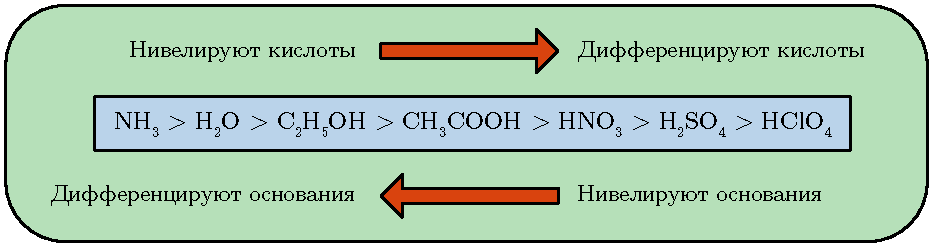
\includegraphics[width=13cm]{figs/acid_and_base_strength/relative_strength_of_acids_and_bases.pdf}
    \caption{Нивелирующие и дифференцирующие растворители.}
    \label{fig:relative_strength_of_acids_and_bases}
\end{figure}

\subsection*{Самые сильные и слабые кислоты и основания в водном растворе}

Какая кислота является самой сильной в водном растворе? Поскольку протонированию всегда подвергаются молекулы растворителя, которые затем переносят протон между собой, то самой сильной кислотой в водном растворе является ион гидроксония \ce{H3O^+}.

Поскольку \ce{H3O^+} является предельной кислотой, способной существовать в воде, его константу кислотности по определению принимают за 1 ($\text{p}K_a(\ce{H3O^+}) = 0$) для удобства построения водной шкалы. Формально это соответствует равновесию переноса протона между идентичными частицами:

\reaction*{H3O^+ + H2O <--> H2O + H3O^+{.}}

Что будет происходить в воде с кислотами, у которых $\text{p}K_a < 0$? Очевидно, они будут полностью диссоциированы, и в растворе не будет молекул исходной кислоты, поскольку в соответствии с соотношением

\begin{equation*}
    K_a = \frac{K_w}{K_b}
\end{equation*}

сопряжённые основания, которые образуются при диссоциации этих кислот, будут более слабыми, чем вода, и поэтому практически не протонируются. Поэтому кислотность данных кислот будет определяться исключительно ионами гидроксония, образовавшимися при их диссоциации, то есть кислоты перестанут различаться (будет наблюдаться нивелирующий эффект воды для сильных кислот).

Таким образом, разбавленные растворы сильных кислот в воде не отличаются по кислотности друг от друга.

Заметьте, что иону гидроксония, как самой сильной кислоте в водном растворе, соответствует сопряжённое основание~--- вода, которое будет являться \emph{предельно слабым} основанием в контексте нивелирующего эффекта для сильных кислот, потому что любое основание, образующееся при диссоциации кислот с $\text{p}K_a < 0$, будет слабее него. Рассчитаем константу основности воды\footnote{Не забываем, что значение $K_w = \num{e-14}$ справедливо при \qty{25}{\degreeCelsius}.}:

\begin{equation*}
    K_b(\ce{H2O}) = \frac{K_w}{K_a(\ce{H3O^+})} = \frac{\num{e-14}}{1} = \num{e-14}.
\end{equation*}

Все основания с $K_b < \num{e-14}$ почти не будут протонироваться в водных растворах.

Самым сильным основанием в водных растворах является гидроксид-ион \ce{OH^-}. Сопряжённая c данным основанием кислота~--- вода~--- является условно самой слабой кислотой в водном растворе, которая может диссоциировать. Константа кислотности воды будет равна:

\begin{equation*}
    K_a(\ce{H2O}) = \frac{K_w}{K_b(\ce{OH^-})} = \frac{\num{e-14}}{1} = \num{e-14}.
\end{equation*}

Все кислоты с $K_a < \num{e-14}$ почти не будут диссоциировать в водном растворе.

Основания, более сильные, чем гидроксид-ион (такие соединения, как амиды, гидриды, алкоголяты щелочных металлов и т.~п.) не могут существовать в растворе, потому что необратимо протонируются водой с образованием гидроксид-ионов:

\reaction*{C2H5ONa + H2O -> C2H5OH + OH^-{.}}

Таким образом, относительное распределение кислот и оснований в водном растворе можно представить в виде следующих схем (рис.~\ref{fig:acid_strength_scale} и~\ref{fig:base_strength_scale}).

\begin{figure}[htbp]
    \centering
    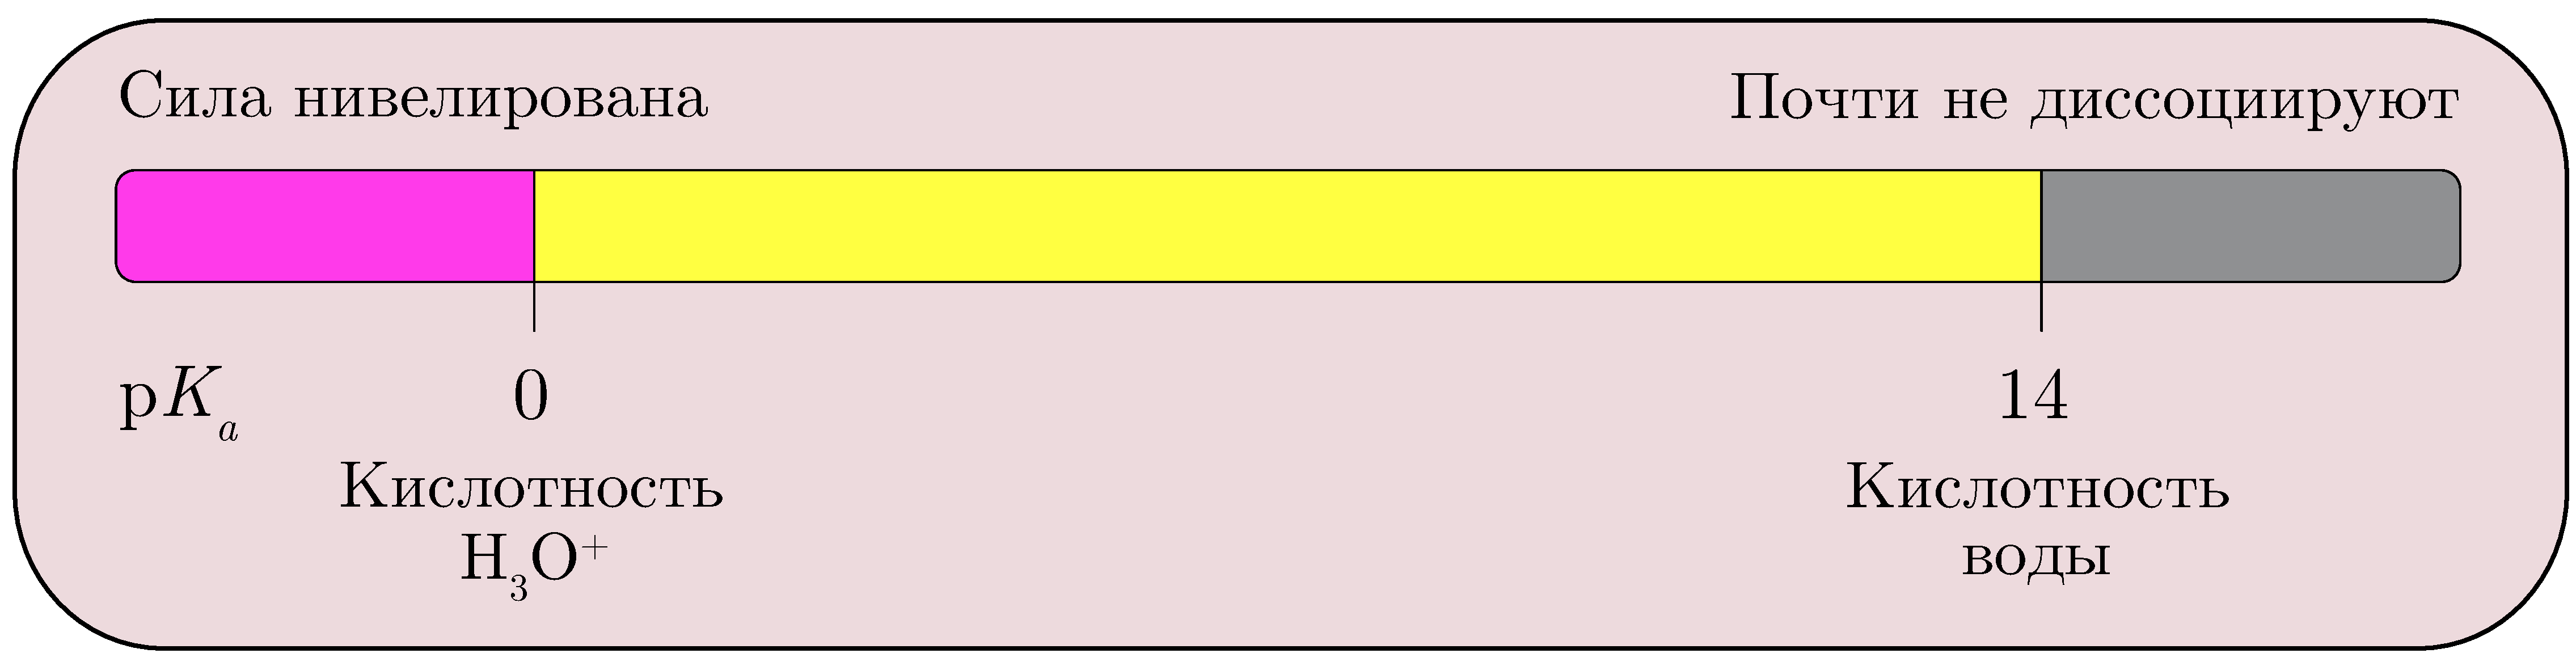
\includegraphics[width=13cm]{figs/acid_and_base_strength/acid_strength_scale.pdf}
    \caption{Шкала силы кислот в водном растворе.}
    \label{fig:acid_strength_scale}
\end{figure}

\begin{figure}[htbp]
    \centering
    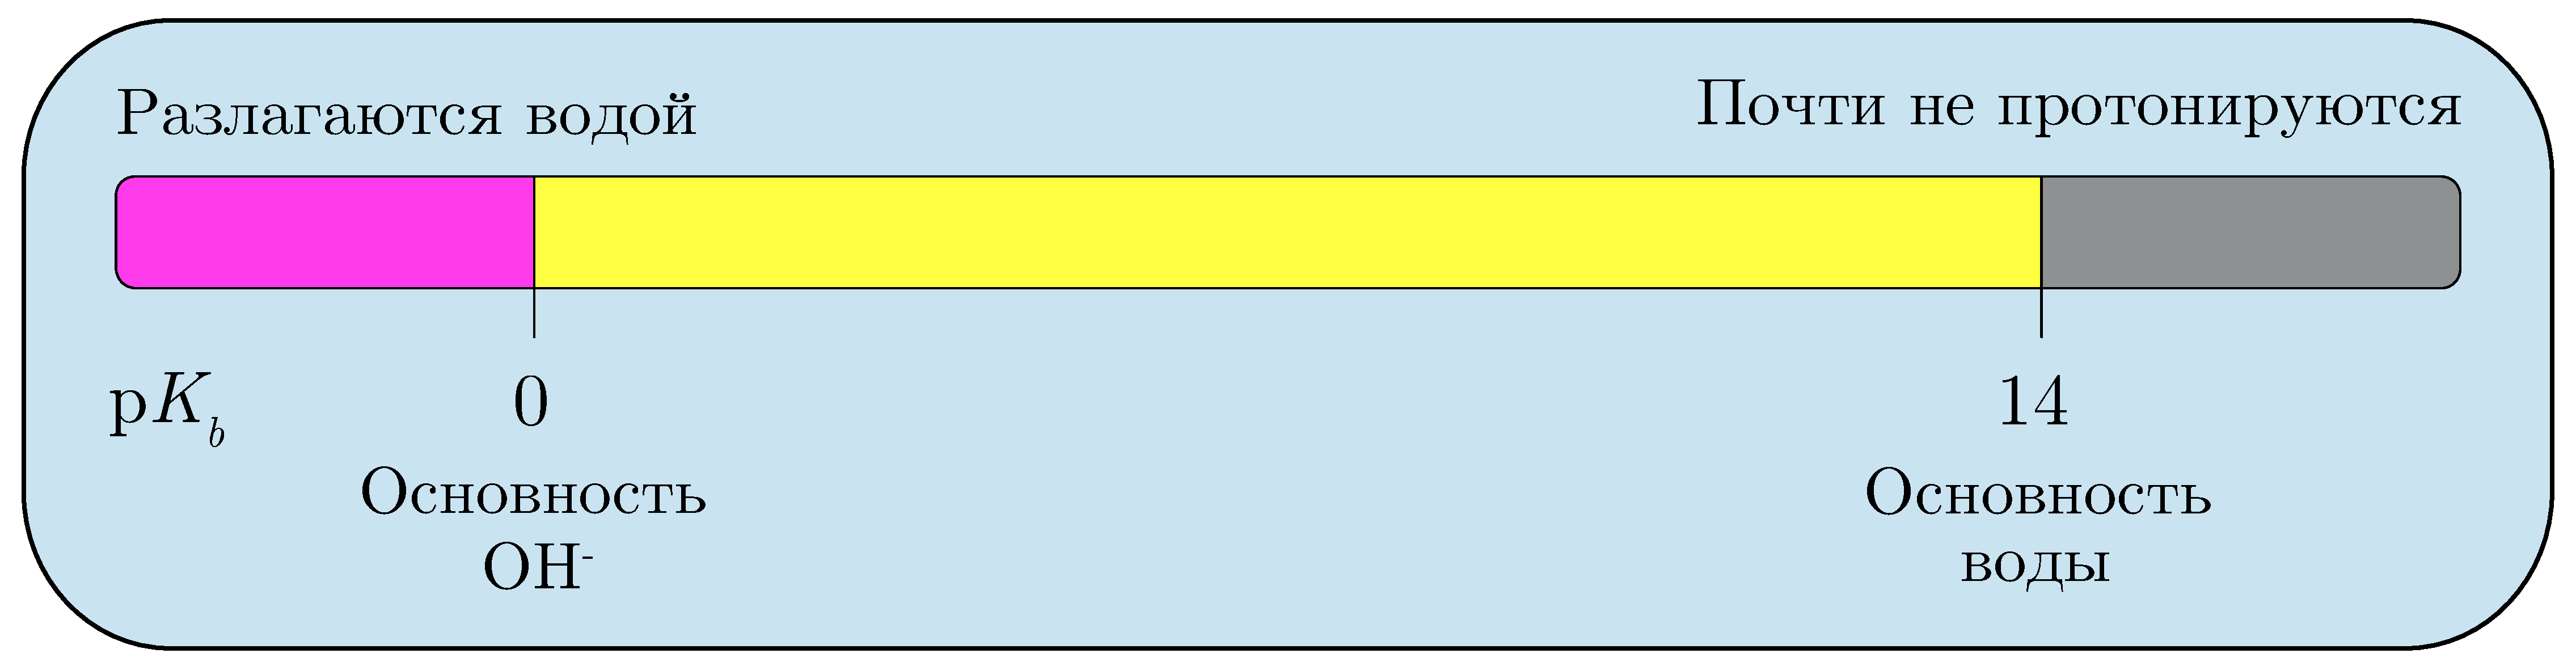
\includegraphics[width=13cm]{figs/acid_and_base_strength/base_strength_scale.pdf}
    \caption{Шкала силы оснований в водном растворе.}
    \label{fig:base_strength_scale}
\end{figure}

\begin{problem}{}{acid_and_base_strength1}
    Чистую уксусную кислоту называют <<ледяная>> по способу её получения. Водный раствор уксусной кислоты начинают замораживать, при этом первыми появляются кристаллы уксусной кислоты ($t_{\text{пл}} = \qty{16,8}{\degreeCelsius}$) а не воды, которые собирают и затем размораживают для получения чистой уксусной кислоты. Почему ледяная уксусная кислота очень плохо проводит электрический ток, однако при внесении в неё даже небольших количеств воды становится сильным электролитом?
    \begin{sol}{\ref{prob:acid_and_base_strength1}}
        Уксусная кислота гораздо более сильная кислота, чем вода, но более слабое основание. Поэтому в чистых веществах константы автопротолиза уксусной кислоты и воды близки и электропроводность одинаково низкая. Однако при добавлении в чистую уксусную кислоту воды~--- более сильного основания, чем сама кислота, последняя начинает проявлять свои кислотные свойства, протонируя воду. Степень диссоциации растёт, диэлектрическая проницаемость среды увеличивается, ионы лучше разделяются, поэтому электропроводность резко возрастает.
    \end{sol}
\end{problem}

\begin{problem}{}{acid_and_base_strength2}
    Какие из перечисленных растворителей будут сильнее дифференцировать кислоты, чем вода: а) \ce{CS2}; б) \ce{H2SO4}; в) ${\ce{NH3}}_{\text{(ж)}}$; г) \ce{CH3COOH}; д) \ce{C2H5OH}; е) \ce{SO2}?
    \begin{sol}{\ref{prob:acid_and_base_strength2}}
        Дифференцируют кислоты вещества с меньшей основностью, чем вода: б, г, е.
    \end{sol}
\end{problem}

\begin{problem}{}{acid_and_base_strength3}
    Какие растворители хорошо нивелируют основания:\\ а) \ce{H2SO4}; б) ${\ce{NH3}}_{\text{(ж)}}$; в) \ce{CH3COOH}; г) \ce{H2O}?
    \begin{sol}{\ref{prob:acid_and_base_strength3}}
        а, в (и г для сильных оснований). Нивелирующий эффект для оснований проявляют растворители с выраженными кислотными свойствами, так как они легко протонируют любые основания, превращая их в сопряжённое основание растворителя. $\ce{NH3}$ является основным растворителем и, напротив, дифференцирует основания.
    \end{sol}
\end{problem}

\begin{problem}{}{acid_and_base_strength4}
    Что будет являться самой сильной кислотой и самым сильным основанием в жидком аммиаке?
    \begin{sol}{\ref{prob:acid_and_base_strength4}}
        Самой сильной кислотой будет ион аммония \ce{NH4^+}, самым сильным основанием~--- амид-ион \ce{NH2^-}. Вообще, в любом растворителе \ce{HSol} самой сильной кислотой будет являться ион \ce{H2Sol^+}, называемый ионом лиония, а самым сильным основанием~--- ион \ce{Sol^-}, который называют лиат-ионом.
    \end{sol}
\end{problem}

\begin{problem}{}{acid_and_base_strength5}
    Назовите самую слабую кислоту, способную диссоциировать и самое слабое основание, способное протонироваться в этиловом спирте.
    \begin{sol}{\ref{prob:acid_and_base_strength5}}
        Сам этиловый спирт.
    \end{sol}
\end{problem}

\begin{problem}{}{acid_and_base_strength6}
    У вас есть два сильных основания, оба из которых реагируют с водой. Опишите общую схему, в соответствии с которой вы сумеете определить, какой из них является более основным.
    \begin{sol}{\ref{prob:acid_and_base_strength6}}
        \begin{enumerate}[label=\arabic*)]
            \item Подбираем растворитель с высокой основностью, в котором растворяются оба вещества.
            \item Определяем, какое из этих веществ диссоциирует сильнее, например, измерив величину электропроводности растворов с одинаковой молярной концентрацией.
            \item Вещество, раствор которого будет иметь большую электропроводность, будет более основным.
            \item В случае, если электропроводности не будут различаться, растворитель подобран неверно и пробуем с другим растворителем.
        \end{enumerate}
    \end{sol}
\end{problem}

\begin{problem}{}{acid_and_base_strength7}
    Как вы считаете, можно ли использовать константу автопротолиза растворителя в качестве показателя способности к нивелирующему и дифференцирующему эффекту?
    \begin{sol}{\ref{prob:acid_and_base_strength7}}
        Нельзя, поскольку для оценки способности растворителя к нивелирующему и дифференцирующему эффекту нам важна кислотность и основность растворителя, а константа автопротолиза указывает только на то, насколько легко растворитель генерирует собственные ионы. Или, другими словами, константа автопротолиза определяет ширину шкалы кислотности растворителя, но не его сродство к протону относительно конкретных растворённых веществ. 
    \end{sol}
\end{problem}

\begin{problem}{}{acid_and_base_strength8}
    Взглянув на формулу воды \ce{H2O} и вспомнив о её свойствах очень слабой кислоты, можно прийти к выводу, что вода формально является двухосновной кислотой. Однако, хотя для такой двухосновной кислоты, как серная, в растворе зафиксировано образование анионов \ce{SO4^{2-}}, до сих пор не обнаружено образование аниона \ce{O^{2-}} в водных растворах. Почему?
    \begin{sol}{\ref{prob:acid_and_base_strength8}}
        Чтобы оторвать ещё один протон от гидроксид-иона \ce{OH^-} требуется преодолеть притяжение двухзарядного иона \ce{O^{2-}}, что энергетически очень затруднительно. По той же причине в растворе сероводорода практически отсутствуют ионы \ce{S^{2-}}. В серной же кислоте отрыв второго протона происходит от другого атома кислорода, не несущего заряд. Кроме того, ион $\ce{O^{2-}}$ является очень сильным основанием и в воде мгновенно и необратимо гидролизуется: $\ce{O^{2-} + H2O -> 2OH^-}$.

    \end{sol}
\end{problem}

\clearpage

\section{Положение протолитического равновесия}

\hspace*{\parindent}Положение протолитического равновесия смещено в сторону образования более слабой кислоты и более слабого основания.

Покажем, почему это так. Рассмотрим реакцию переноса протона:
\reaction*{HA + B <--> A^- + BH^+{.}}

Константа равновесия данной реакции будет равна:

\begin{equation*}
    K = \frac{[\ce{A^-}][\ce{BH^+}]}{[\ce{HA}][\ce{B}]}{.}
\end{equation*}

Умножим числитель и знаменатель на \ce{[H^+]} и сгруппируем множители:

\begin{equation*}
    K = \frac{[\ce{A^-}][\ce{H^+}]}{[\ce{HA}]} \cdot \frac{[\ce{BH^+}]}{[\ce{B}][\ce{H^+}]} 
      = \frac{K_a(\ce{HA})}{K_a(\ce{BH^+})}{.}
\end{equation*}

Если $K_a(\ce{HA}) > K_a(\ce{BH^+})$, то $K > 1$ и равновесие смещено вправо, то есть в сторону более слабой кислоты $\ce{BH^+}$. Аналогично, умножив числитель и знаменатель на \ce{[OH^-]}, получаем:

\begin{equation*}
    K = \frac{[\ce{BH^+}][\ce{OH^-}]}{[\ce{B}]} \cdot \frac{[\ce{A^-}]}{[\ce{HA}][\ce{OH^-}]} 
      = \frac{K_b(\ce{B})}{K_b(\ce{A^-})}{.}
\end{equation*}

Равновесие смещено в сторону основания с меньшей $K_b$ (более слабого). Прологарифмировав выражение через $K_a$, получим удобную формулу для оценки положения равновесия:

\begin{equation*}
    \fbox{$\displaystyle \lg K = \text{p}K_a(\ce{BH^+}) - \text{p}K_a(\ce{HA})$}.
\end{equation*}

Аналогично для оснований:

\begin{equation*}
    \fbox{$\displaystyle \lg K = \text{p}K_b(\ce{A^-}) - \text{p}K_b(\ce{B})$}.
\end{equation*}

\begin{example}{}{ex:position_of_protolytic_equilibrium1}
    \begin{condition}
        Определите направления смещения равновесия в следующих протолитических реакциях:
        \reaction*{HS^- + H2O <--> H2S + OH^-{,}}
        \reaction*{CO3^{2-} + CH3COOH <--> HCO3^- + CH3COO^-{,}}
        \reaction*{NH4^+ + I^- <--> NH3 + HI{.}}
    \end{condition}

    \medskip

    \textit{Решение.} Положение протолитического равновесия смещено в сторону образования более слабой кислоты и более слабого основания. В первом равновесии в правой части имеется самое сильное основание в водном растворе~--- гидроксид-ион, поэтому положение равновесия будет сдвинуто в сторону более слабого основания~--- гидросульфид-аниона, то есть влево:
    \reaction*{HS^- + H2O <<=> H2S + OH^-{.}}
    Во втором равновесии проще всего сравнить константы кислотности уксусной и угольной (по 2-й ступени) кислот: $K_a(\ce{CH3COOH}) = \num{1,75e-5}$, $K_a(\ce{HCO3^-}) = \num{4,69e-11}$. Уксусная кислота значительно сильнее, поэтому равновесие будет сдвинуто вправо:
    \reaction*{CO3^{2-} + CH3COOH <=>> HCO3^- + CH3COO^-{.}}
    В третьем равновесии имеется иодоводородная кислота~--- одна из самых сильных кислот в водных растворах, поэтому положение равновесия будет сдвинуто влево, в сторону более слабой кислоты (\ce{NH4^+}) и более слабого основания (\ce{I^-}):
    \reaction*{NH4^+ + I^- <<=> NH3 + HI{.}}

\end{example}

\begin{example}{}{ex:position_of_protolytic_equilibrium2}
    \begin{condition}
        Рассчитайте константу равновесия реакции:
        \reaction*{HSO4^- + HCl <--> H2SO4 + Cl^-{.}}
    \end{condition}

    \medskip

    \textit{Решение.} Воспользуемся формулой расчёта константы протолитического равновесия через $\text{p}K_a$ кислот. Из справочника находим значения $\text{p}K_a$ для соляной и серной кислот: $\text{p}K_a(\ce{HCl}) = -7$, $\text{p}K_a(\ce{H2SO4}) = -3$. Рассчитаем константу равновесия:
    \begin{equation*}
        \lg K = \text{p}K_a(\ce{BH^+}) - \text{p}K_a(\ce{HA}) = -3 - (-7) = 4.
    \end{equation*}
    \begin{equation*}
        K = \num{e4}.
    \end{equation*}
    Обратите внимание, что в качестве кислоты \ce{HA} в уравнении протолитического равновесия выступает именно хлороводород~--- именно эта молекула отдаёт протон. Поскольку $K \gg 1$, то положение равновесия в данном случае сильно смещено вправо, что отражает тот факт, что соляная кислота значительно сильнее серной. Вдумчивый читатель может возразить, что в данном случае имеет место нивелирующий эффект воды как растворителя, и будет прав: в разбавленном водном растворе обе кислоты нивелируются до \ce{H3O^+}. Данный расчёт корректен для концентрированных растворов.
\end{example}

\begin{problem}{}{position_of_protolytic_equilibrium1}
    Какие из перечисленных веществ проявляют свойства кислоты в водном растворе: а) \ce{BaCl2}; б) \ce{NaHSO4}; в) \ce{Ca(OH)2}; г) \ce{H2S}; д) \ce{ZnSO4}; е) \ce{Ca3(PO4)2}; ж) \ce{B(OH)3}?
    \begin{sol}{\ref{prob:position_of_protolytic_equilibrium1}}
        Согласно формулировке задачи, вещества должны <<проявлять свойства кислоты в водном растворе>> и не обязательно являться кислотой Брёнстеда в строгом смысле этого слова. Протолитическое равновесие с участием соединения может приводить к тому, что оно будет проявлять свойства кислоты или основания. Например, раствор сульфата цинка имеет кислую реакцию среды из-за того, что в растворе устанавливается протолитическое равновесие
        \reaction*{Zn^{2+} + H2O <--> ZnOH^+ + H^+{.}}
        Правильные ответы: б, г, д, ж.
    \end{sol}
\end{problem}

\begin{problem}{}{position_of_protolytic_equilibrium2}
    Какие из перечисленных веществ проявляют свойства основания в водном растворе: а) \ce{NaOCl}; б) \ce{BaSO4}; в) \ce{NH3}; г) \ce{Sr(OH)2}; д) \ce{NaHCO3}; е) \ce{Na2CO3}; ж) \ce{Ba(OH)2}; з) \ce{K2S}?
    \begin{sol}{\ref{prob:position_of_protolytic_equilibrium2}}
        а, в, г, д, е, ж, з. Гидрокарбонат-ион амфотерен, но его константа основности $K_b = K_w/K_{a1} \approx \num{2,3e-8}$ превышает константу кислотности $K_{a2} \approx \num{4,7e-11}$, поэтому гидролиз преобладает над диссоциацией.
    \end{sol}
\end{problem}

\begin{problem}{}{position_of_protolytic_equilibrium3}
    В какую сторону смещены следующие равновесия:
    \begin{enumerate}[label=\arabic*)]
        \item \ce{NH3 + H2O <=> NH4^+ + OH^-{;}}
        \item \ce{HF + I^- <--> HI + F^-{;}}
        \item \ce{HPO4^{2-} + CH3COOH <--> H2PO4^- + CH3COO^-{;}}
        \item \ce{H2S + OH^- <--> HS^- + H2O{;}}
        \item \ce{HSO3^- + NH3 <--> SO3^{2-} + NH4^+{?}}
    \end{enumerate}
    \begin{sol}{\ref{prob:position_of_protolytic_equilibrium3}}
        Положение протолитического равновесия смещено в сторону образования более слабой кислоты и более слабого основания:
        \begin{enumerate}[label=\arabic*)]
            \item влево;
            \item влево;
            \item вправо;
            \item вправо;
            \item вправо.
        \end{enumerate}
    \end{sol}
\end{problem}

\begin{problem}{}{position_of_protolytic_equilibrium4}
    Рассчитайте константу равновесия для следующей реакции:
    \reaction*{HBr + HSO4^- <--> H2SO4 + Br^-{.}}
    Как вы объясните тот факт, что реакция
    \reaction*{2KBr + H2SO4 -> 2HBr (^) + K2SO4}
    прекрасно протекает при обычных условиях?
    \begin{sol}{\ref{prob:position_of_protolytic_equilibrium4}}
        Рассчитаем константу равновесия используя кислотности серной и бромоводородной кислот:
        \begin{equation*}
            K = \frac{K_a(\ce{HBr})}{K_a(\ce{H2SO4})} = \frac{\num{e9}}{\num{e3}} = \num{e6}.
        \end{equation*}
        Равновесие очень сильно сдвинуто вправо, однако указанная реакция протекает, поскольку образующийся бромоводород удаляется из реакционной смеси. Это общее правило, согласно которому менее летучие кислоты вытесняют более летучие из их солей несмотря на константы кислотности.

        В реальных условиях концентрированная \ce{H2SO4} частично окисляет \ce{HBr} до \ce{Br2}, поэтому для чистого получения бромоводорода на практике используют \ce{H3PO4}.
    \end{sol}
\end{problem}

\clearpage

\section[Материальный баланс. Электронейтральность]{Материальный баланс. Условие электронейтральности}

\subsection*{Материальный баланс}

Правило материального баланса в растворе звучит следующим образом: при протекании реакции в изолированной системе общее число атомов в реагирующих веществах остаётся постоянным. Это означает, что число атомов определённого типа до реакции равно числу атомов этого типа и после реакции.

Например, при диссоциации сернистой кислоты \ce{H2SO3} в растворе присутствуют продукты диссоциации по первой ступени, по второй ступени и сама недиссоциировавшая кислота\footnote{На самом деле, в водном растворе сернистая кислота существует преимущественно в виде гидрата \ce{SO2*H2O}, а не молекул \ce{H2SO3}, однако при записи уравнений такой формализм допустим.}:

\reaction*{H2SO3 <--> H^+ + HSO3^-{;}}
\reaction*{HSO3^- <--> H^+ + SO3^{2-}{.}}

Общая концентрация сернистой кислоты (определяемая аналитически) складывается из концентраций всех частиц в растворе, содержащих атомы серы:

\begin{equation*}
    c(\ce{H2SO3}) = [\ce{H2SO3}] + [\ce{HSO3^-}] + [\ce{SO3^{2-}}].
\end{equation*}

Материальный баланс можно записать и с учётом других атомов, но в этом случае нужно помнить, что частицы, концентрация которых входит в материальный баланс, могут образовываться и из других источников.

Если в частице содержится больше, чем один атом, по которому составляется баланс, нужно умножить концентрацию частицы на количество атомов. Например, тот же баланс мы могли бы записать по атомам водорода:

\begin{equation*}
    2c(\ce{H2SO3}) = 2[\ce{H2SO3}] + [\ce{HSO3^-}] + [\ce{H^+}].
\end{equation*}

Однако данная запись будет верна только при определённых приближениях, поскольку ионы водорода могут образовываться в растворе не только из сернистой кислоты, но и при диссоциации молекул воды или других веществ. В водных растворах материальный баланс практически всегда составляют по <<центральному>> атому (\ce{S}, \ce{C}, \ce{N}, металл и т.~д.), а не по водороду или кислороду, поскольку вклад молекул воды в их общее количество на много порядков превышает вклад растворённых веществ.

При составлении материального баланса нужно обязательно учесть \emph{все} частицы, в которых содержатся интересующие нас атомы.

Например, в ацетатном буфере, представляющем собой водный раствор уксусной кислоты и ацетата натрия, материальный баланс по атомам углерода можно записать так:

\begin{equation*}
    c_{\text{исх}}(\ce{CH3COOH}) + c_{\text{исх}}(\ce{CH3COONa}) = [\ce{CH3COOH}] + [\ce{CH3COO^-}].
\end{equation*}

Необходимо также помнить, что ионы, образующиеся при диссоциации, могут сами вступать в дальнейшие превращения, поэтому их концентрация может быть ниже, чем может показаться. Например, при диссоциации солей могут образовываться анионы, которые сами могут участвовать в протолитическом равновесии, например:

\reaction*{NaClO <--> Na^+ + ClO^-{;}}
\reaction*{ClO^- + H2O <--> HClO + OH^-{.}}

В этом случае нельзя записать следующие равенства:

\begin{equation*}
    c(\ce{NaClO}) = [\ce{ClO^-}],
\end{equation*}
\begin{equation*}
    [\ce{ClO^-}] = [\ce{Na^+}].
\end{equation*}

В данном случае необходимо учитывать концентрацию всех частиц, содержащих атомы хлора:

\begin{equation*}
    c(\ce{NaClO}) = [\ce{ClO^-}] + [\ce{HClO}].
\end{equation*}

\subsection*{Условие электронейтральности}

В любых растворах выполняется \textbf{условие электронейтральности}\label{term:electro_neutrality_condition}\index{условие электронейтральности}: в единице объёма раствора сумма положительных зарядов равна сумме отрицательных зарядов, то есть

\begin{equation*}
    \fbox{$\displaystyle\sum_{i = 1}^{n} c_iz_i = 0$},  
\end{equation*}

где $c_i$~--- концентрация $i$-го иона, а $z_i$~--- его заряд.

Смысл условия электронейтральности в том, что в растворе для любой заряженной частицы всегда найдутся другие заряженные частицы с противоположным знаком заряда, компенсирующие её заряд.

Не существует растворов, в которых были бы только отрицательно или только положительно заряженные ионы. Например, при диссоциации нитрата натрия образуются частицы, суммарный заряд которых равен нулю:

\reaction*{NaNO3 <--> Na^+ + NO3^-{.}}

При этом происходит также диссоциация молекул воды:

\reaction*{H2O <--> H^+ + OH^-{.}}

Уравнение электронейтральности для данного раствора будет записано так:

\begin{equation*}
    [\ce{Na^+}] + [\ce{H^+}] = [\ce{NO3^-}] + [\ce{OH^-}].
\end{equation*}

Если при диссоциации образуется частица с зарядом больше единичного, то концентрация этой частицы должна быть умножена на величину её заряда, поскольку наличие данного иона в растворе приводит к увеличению концентрации частиц с единичным зарядом и противоположным знаком:

\reaction*{BaCl2 <--> Ba^{2+} + 2Cl^-{;}}
\reaction*{H2O <--> H^+ + OH^-{.}}

\begin{equation*}
    2[\ce{Ba^{2+}}] + [\ce{H^+}] = [\ce{Cl^-}] + [\ce{OH^-}].
\end{equation*}

Необходимо учесть все присутствующие в растворе ионы, если только их концентрация не пренебрежимо мала, например:

\reaction*{NaHSO4 <--> Na^+ + HSO4^-{;}}
\reaction*{HSO4^- <--> H^+ + SO4^{2-}{;}}
\reaction*{H2O <--> H^+ + OH^-{.}}

\begin{equation*}
    [\ce{Na^+}] + [\ce{H^+}] = [\ce{HSO4^-}] + 2[\ce{SO4^{2-}}] + [\ce{OH^-}].
\end{equation*}

Обратите внимание, что для данных равновесий равенства $[\ce{Na^+}] = [\ce{HSO4^-}]$, $[\ce{H^+}] = [\ce{SO4^{2-}}]$ и $[\ce{H^+}] = [\ce{OH^-}]$ будут неверными.

\begin{example}{}{ex:material_balance_electro_neutrality_condition1}
    \begin{condition}
        Напишите уравнение материального баланса для раствора серной кислоты.
    \end{condition}

    \medskip

    \textit{Решение.} При диссоциации серной кислоты в растворе присутствуют следующие частицы: \ce{SO4^{2-}}, \ce{HSO4^-}, \ce{H^+} и \ce{H2SO4}. Общая концентрация серной кислоты будет равна:
    \begin{equation*}
        c(\ce{H2SO4}) = [\ce{H2SO4}] + [\ce{HSO4^-}] + [\ce{SO4^{2-}}];
    \end{equation*}
    В водном растворе $[\ce{H2SO4}] \approx 0$ из-за сильной первой ступени диссоциации, но в уравнении баланса она сохраняется для общности записи.
\end{example}

\begin{example}{}{ex:material_balance_electro_neutrality_condition2}
    \begin{condition}
        Составьте уравнение электронейтральности для водного раствора хлорида лития.
    \end{condition}

    \medskip

    \textit{Решение.} Для составления уравнения электронейтральности нужно разнести концентрации носителей положительных и отрицательных зарядов в левую и правую части уравнения. В растворе хлорида лития присутствуют положительно заряженные ионы лития и ионы гидроксония, образующиеся при автопротолизе воды. Отрицательно заряженными ионами являются хлорид-анионы и гидроксид-ионы, поэтому уравнение электронейтральности выглядит так:
    \begin{equation*}
        [\ce{Li^+}] + [\ce{H^+}] = [\ce{Cl^-}] + [\ce{OH^-}].
    \end{equation*}
\end{example}

\begin{example}{}{ex:material_balance_electro_neutrality_condition3}
    \begin{condition}
        Составьте уравнение электронейтральности для водного раствора нитрата магния.
    \end{condition}

    \medskip

    \textit{Решение.} При диссоциации нитрата магния на каждый двухзарядный ион магния образуется два однозарядных нитрат-аниона, что нужно учесть при составлении уравнения. Поэтому концентрацию ионов магния нужно удвоить. Кроме того, ионы магния в растворе подвергаются обратимому гидролизу, приводящему к кислой среде раствора и наличию частиц \ce{MgOH^+}:
    \reaction*{Mg^{2+} + H2O <--> MgOH^+ + H^+{.}}
    Поэтому уравнение электронейтральности записываем так (из-за низкой концентрации гидроксид-ионов ею пренебрегаем):
    \begin{equation*}
        2[\ce{Mg^{2+}}] + [\ce{MgOH^+}] + [\ce{H^+}] = [\ce{NO3^-}].
    \end{equation*}
\end{example}

\begin{example}{}{ex:material_balance_electro_neutrality_condition4}
    \begin{condition}
        Какова концентрация сульфит-ионов в \qty{0,005}{\M} растворе сернистой кислоты при $\text{pH} = 5$?
    \end{condition}

    \medskip

    \textit{Решение.} Чтобы выразить концентрацию сульфит-ионов составим материальный баланс для раствора сернистой кислоты:
    \begin{equation*}
        c(\ce{H2SO3}) = [\ce{H2SO3}] + [\ce{HSO3^-}] + [\ce{SO3^{2-}}].
    \end{equation*}
    Затем из выражения для констант кислотности сернистой кислоты выразим концентрации молекулярной кислоты и гидросульфит-аниона и подставим в уравнение материального баланса:
    \begin{align*}
        K_a(\ce{HSO3^-}) &= \frac{[\ce{H^+}][\ce{SO3^{2-}}]}{[\ce{HSO3^-}]}
        \quad\Longrightarrow\quad
        [\ce{HSO3^-}] = \frac{[\ce{H^+}][\ce{SO3^{2-}}]}{K_a(\ce{HSO3^-})}, \\[0.8ex]
        K_a(\ce{H2SO3}) &= \frac{[\ce{H^+}][\ce{HSO3^-}]}{[\ce{H2SO3}]}
        \quad\Longrightarrow\quad
        [\ce{H2SO3}] = \frac{[\ce{H^+}][\ce{HSO3^-}]}{K_a(\ce{H2SO3})}
        = \frac{[\ce{H^+}]^2[\ce{SO3^{2-}}]}{K_a(\ce{H2SO3})K_a(\ce{HSO3^-})}.
    \end{align*}
    \begin{align*}
        c(\ce{H2SO3}) &= \frac{[\ce{H^+}]^2[\ce{SO3^{2-}}]}{K_a(\ce{H2SO3})K_a(\ce{HSO3^-})}
        + \frac{[\ce{H^+}][\ce{SO3^{2-}}]}{K_a(\ce{HSO3^-})}
        + [\ce{SO3^{2-}}] \\[0.5ex]
        &= [\ce{SO3^{2-}}]\left(
            \frac{[\ce{H^+}]^2}{K_a(\ce{H2SO3})K_a(\ce{HSO3^-})}
            + \frac{[\ce{H^+}]}{K_a(\ce{HSO3^-})}
            + 1
        \right).
    \end{align*}
    \begin{equation*}
        [\ce{SO3^{2-}}] = \frac{c(\ce{H2SO3})}{
            \dfrac{[\ce{H^+}]^2}{K_a(\ce{H2SO3})K_a(\ce{HSO3^-})}
            + \dfrac{[\ce{H^+}]}{K_a(\ce{HSO3^-})} + 1
        }.
    \end{equation*}
    \begin{equation*}
        [\ce{SO3^{2-}}] = \frac{\num{5e-3}}{
            \dfrac{(\num{e-5})^2}{\num{1,58e-2} \cdot \num{6,3e-8}}
            + \dfrac{\num{e-5}}{\num{6,3e-8}} + 1
        } = \qty{3,13e-5}{\M}.
    \end{equation*}
\end{example}

\begin{problem}{}{material_balance_electro_neutrality_condition1}
    Напишите уравнение материального баланса для водного раствора ортофосфорной кислоты.
    \begin{sol}{\ref{prob:material_balance_electro_neutrality_condition1}}
        Уравнение баланса по частицам, содержащим фосфор:
        \begin{equation*}
            c(\ce{H3PO4}) = [\ce{H3PO4}] + [\ce{H2PO4^-}] + [\ce{HPO4^{2-}}] + [\ce{PO4^{3-}}].
        \end{equation*}
    \end{sol}
\end{problem}

\begin{problem}{}{material_balance_electro_neutrality_condition2}
    Напишите уравнение материального баланса для водного раствора гидросульфида натрия.
    \begin{sol}{\ref{prob:material_balance_electro_neutrality_condition2}}
        Гидросульфид-ион как достаточно сильное основание участвует в протолитическом равновесии с молекулами воды:
        \reaction*{HS^- + H2O <--> H2S + OH^-{.}}
        Гидросульфид-ион мог бы диссоциировать по кислотному типу:
        \reaction*{HS^- <--> H^+ + S^{2-}{,}}
        однако $\text{p}K_{a2}(\ce{H2S}) \approx 17\text{--}19$, поэтому концентрация $\ce{S^{2-}}$ пренебрежимо мала и ею можно пренебречь. Уравнение материального баланса можно записать так:
        \begin{equation*}
            c(\ce{NaHS}) = [\ce{HS^-}] + [\ce{H2S}].
        \end{equation*}
    \end{sol}
\end{problem}

\begin{problem}{}{material_balance_electro_neutrality_condition3}
    Напишите уравнение материального баланса по оксалат-ионам (анионам щавелевой кислоты) и атомам водорода для раствора щавелевой кислоты. Диссоциацией воды пренебречь.
    \begin{sol}{\ref{prob:material_balance_electro_neutrality_condition3}}
        Не учитывая диссоциацию воды:
        \begin{equation*}
            c(\ce{H2C2O4}) = [\ce{H2C2O4}] + [\ce{HC2O4^-}] + [\ce{C2O4^{2-}}],
        \end{equation*}
        \begin{equation*}
            2c(\ce{H2C2O4}) = [\ce{H^+}] + [\ce{HC2O4^-}] + 2[\ce{H2C2O4}].
        \end{equation*}
    \end{sol}
\end{problem}

\begin{problem}{}{material_balance_electro_neutrality_condition4}
    Составьте уравнение электронейтральности для водного раствора хлорида натрия.
    \begin{sol}{\ref{prob:material_balance_electro_neutrality_condition4}}
        Источниками ионов в растворе являются растворённый хлорид натрия и автопротолиз воды:
        \begin{equation*}
            [\ce{Na^+}] + [\ce{H^+}] = [\ce{Cl^-}] + [\ce{OH^-}].
        \end{equation*}
    \end{sol}
\end{problem}

\begin{problem}{}{material_balance_electro_neutrality_condition5}
    Составьте уравнение электронейтральности для водного раствора фосфата калия.
    \begin{sol}{\ref{prob:material_balance_electro_neutrality_condition5}}
        Фосфат-ион является достаточно сильным основанием и ступенчато гидролизуется, поэтому в баланс зарядов необходимо включить все его заряженные формы. Необходимо помнить о том, что концентрацию трёхзарядного фосфат-аниона нужно утроить:
        \begin{equation*}
            [\ce{K^+}] + [\ce{H^+}] = [\ce{OH^-}] + [\ce{H2PO4^-}] + 2[\ce{HPO4^{2-}}] + 3[\ce{PO4^{3-}}].
        \end{equation*}
    \end{sol}
\end{problem}

\begin{problem}{}{material_balance_electro_neutrality_condition6}
    Составьте уравнение электронейтральности для водного раствора сульфата аммония в двух вариантах: если можно пренебречь диссоциацией воды и если нельзя.
    \begin{sol}{\ref{prob:material_balance_electro_neutrality_condition6}}
        Ионы аммония участвуют в протолитическом равновесии с водой, создавая избыток ионов водорода:
        \reaction*{NH4^+ + H2O <--> NH3 + H^+{.}}
        Поэтому, пренебрегая диссоциацией воды, получим уравнение:
        \begin{equation*}
            [\ce{NH4^+}] + [\ce{H^+}] = 2[\ce{SO4^{2-}}].
        \end{equation*}
        Если диссоциацией воды не пренебрегать, то мы должны включить в уравнение ещё и гидроксид-ионы:
        \begin{equation*}
            [\ce{NH4^+}] + [\ce{H^+}] = 2[\ce{SO4^{2-}}] + [\ce{OH^-}].
        \end{equation*}
    \end{sol}
\end{problem}

\begin{problem}{}{material_balance_electro_neutrality_condition7}
    $\bigstar$ pH некоторого раствора, содержащего \qty{0,001}{\M} фтороводородной кислоты, равен 5 (pH раствора доведён до 5 добавлением щёлочи). Рассчитайте концентрацию фторид-ионов в нём.
    \begin{sol}{\ref{prob:material_balance_electro_neutrality_condition7}}
        Составим материальный баланс для фтороводородной кислоты:
        \begin{equation*}
            c(\ce{HF}) = [\ce{HF}] + [\ce{F^-}].
        \end{equation*}
        Выразим равновесную концентрацию непродиссоциировавшей кислоты из константы диссоциации и подставим в уравнение материального баланса, затем выразим $[\ce{F^-}]$:
        \begin{equation*}
            K_a(\ce{HF}) = \frac{[\ce{H^+}][\ce{F^-}]}{[\ce{HF}]}
            \quad\Longrightarrow\quad
            [\ce{HF}] = \frac{[\ce{H^+}][\ce{F^-}]}{K_a(\ce{HF})}.
        \end{equation*}
        \begin{equation*}
            c(\ce{HF}) = [\ce{HF}] + [\ce{F^-}]
            = \frac{[\ce{H^+}][\ce{F^-}]}{K_a(\ce{HF})} + [\ce{F^-}]
            = \left(\frac{[\ce{H^+}]}{K_a(\ce{HF})} + 1\right)[\ce{F^-}].
        \end{equation*}
        \begin{equation*}
            [\ce{F^-}] = \frac{c(\ce{HF})}{\dfrac{[\ce{H^+}]}{K_a(\ce{HF})} + 1}
            = \frac{c(\ce{HF})}{\dfrac{10^{-\text{pH}}}{K_a(\ce{HF})} + 1}
            = \frac{\num{e-3}}{\dfrac{\num{e-5}}{\num{6,61e-4}} + 1}
            = \qty{9,85e-4}{\M}.
        \end{equation*}
    \end{sol}
\end{problem}

\clearpage

\section[Степень диссоциации]{Степень диссоциации.\\Закон разбавления Оствальда}

В растворах слабых электролитов значительная часть молекул находится в недиссоциированном состоянии, если только раствор не является очень разбавленным.

\textbf{Степенью диссоциации}\label{term:degree_of_dissociation}\index{степень диссоциации} $\alpha$ называют отношение числа продиссоциировавших молекул растворённого вещества $n$ к общему числу молекул вещества $N$:

\begin{equation*}
    \fbox{$\displaystyle\alpha = \frac{n}{N}$}.
\end{equation*}

Рассмотрим диссоциацию слабой кислоты \ce{HA} с общей концентрацией, равной $c_{\ce{HA}}$:

\reaction*{HA <--> H^+ + A^-{.}}

$[\ce{H^+}] = [\ce{A^-}] = \alpha c_{\ce{HA}}$, $[\ce{HA}] = c_{\ce{HA}} - \alpha c_{\ce{HA}}$, откуда:

\begin{equation*}
    K_a(\ce{HA}) = \frac{\alpha c_{\ce{HA}} \cdot \alpha c_{\ce{HA}}}{c_{\ce{HA}} - \alpha c_{\ce{HA}}}
    = \fbox{$\displaystyle\frac{{\alpha}^2}{1 - \alpha}c_{\ce{HA}}$}.
\end{equation*}

Данное выражение называют \textbf{законом разбавления Оствальда}\label{term:Ostwalds_dilution_law}\index{закон разбавления Оствальда}. Если растворённое вещество диссоциирует очень слабо, то можно принять, что $1 - \alpha \approx 1$, и тогда

\begin{equation*}
    \alpha \approx \sqrt{\frac{K_a(\ce{HA})}{c_{\ce{HA}}}}.
\end{equation*}

Эта упрощённая формула даёт приемлемую точность, если $\alpha < \num{0,05}$ (\qty{5}{\percent}), однако если степень диссоциации выше, то для её нахождения необходимо решить квадратное уравнение относительно $\alpha$:

\begin{equation*}
    \alpha = \frac{-K_a(\ce{HA}) + \sqrt{(K_a(\ce{HA}))^2 + 4c_{\ce{HA}}K_a(\ce{HA})}}{2c_{\ce{HA}}}.
\end{equation*}

В случае слабых оснований (наподобие аммиака) или анионов солей слабых кислот говорят не о диссоциации, поскольку основание формально не диссоциирует, а о протолитическом равновесии с участием растворителя, например:

\reaction*{CH3COO^- + H2O <--> CH3COOH + OH^-{.}}

Поэтому в этом случае используют термин не <<степень диссоциации>>, а <<\textbf{степень гидролиза}\label{term:degree_of_hydrolysis}\index{степень гидролиза}>>, которую обозначают $h$\footnote{Термин <<степень гидролиза>> ($h$) сохраняется по исторической традиции (теория Аррениуса) и допускается IUPAC. С позиций теории Брёнстеда–Лоури это частный случай протолитического равновесия, поэтому современное название данного термина~--- <<степень протолиза>>. Не путайте его с \emph{протеолизом}~--- ферментативным расщеплением белков.}. Расчёты в этом случае проводятся совершенно аналогично. 

Необходимо чётко понимать, что расчёты с использованием констант равновесий, которые выражаются через концентрации веществ, можно проводить только для определённого диапазона концентраций растворённого вещества. Дело в том, что для вывода формул используется приближение \emph{предельно разбавленного раствора}, в котором можно пренебречь электростатическим взаимодействием между ионами. Для концентрированных растворов это не так, и свойства растворов начинают сильно отличаться от идеальных. В целом можно считать, что расчёты по приведённым здесь и далее формулам можно проводить для растворов с концентрацией растворённого вещества менее \qty{0,1}{\M}.

\begin{problem}{}{degree_of_dissociation1}
    Как увеличить степень диссоциации слабого электролита? Как уменьшить?
    \begin{sol}{\ref{prob:degree_of_dissociation1}}
        Для большинства слабых кислот и оснований диссоциация эндотермична, поэтому степень диссоциации можно увеличить, нагревая раствор, а уменьшить ~--- охлаждая.
        
        Кроме того, внесение в раствор соли с общим ионом (например, добавление ацетата натрия в раствор уксусной кислоты) сдвигает равновесие реакции и подавляет диссоциацию.

        Также при разбавлении степень диссоциации увеличивается, а при концентрировании раствора~--- уменьшается.
    \end{sol}
\end{problem}

\begin{problem}{}{degree_of_dissociation2}
    При растворении некоторого вещества в воде из 500 молекул вещества 20 продиссоциировало. Определите степень диссоциации.
    \begin{sol}{\ref{prob:degree_of_dissociation2}}
        По определению степени диссоциации:
        \begin{equation*}
            \alpha = \frac{n}{N} = \frac{20}{500} = \num{0,04} \, (\qty{4}{\percent}).
        \end{equation*}
    \end{sol}
\end{problem}

\begin{problem}{}{degree_of_dissociation3}
    В \qty{5}{\l} воды растворили \qty{0,02}{\mole} некоторого вещества, из которого \qty{0,0002}{\mole} распалось на ионы. Определите степень диссоциации и тип электролита.
    \begin{sol}{\ref{prob:degree_of_dissociation3}}
        Количество вещества пропорционально числу частиц в нём, поэтому:
        \begin{equation*}
            \alpha = \frac{n}{N} = \frac{\num{0,0002}}{\num{0,02}} = \num{0,01} \, (\qty{1}{\percent}).
        \end{equation*}
        При этом для определения степени диссоциации объём раствора не имеет значения, важна лишь доля продиссоциировавших частиц. Диссоциирует незначительная часть растворённого вещества, поэтому данное вещество можно отнести к слабым электролитам.
    \end{sol}
\end{problem}

\begin{problem}{}{degree_of_dissociation4}
    Подумайте и объясните, в чём, по вашему мнению, причина того, что степень диссоциации любого электролита увеличивается при разбавлении раствора?
    \begin{sol}{\ref{prob:degree_of_dissociation4}}
        Причина увеличения степени диссоциации при разбавлении раствора статистическая. В более разбавленном растворе ионы более удалены друг от друга и вероятность их встречи (и рекомбинации обратно в недиссоциированное соединение) меньше.

        С точки зрения принципа Ле Шателье, разбавление уменьшает концентрации всех частиц, и равновесие смещается в сторону большего числа частиц (ионов).
    \end{sol}
\end{problem}

\begin{problem}{}{degree_of_dissociation5}
    Рассчитайте степень диссоциации чистой воды.
    \begin{sol}{\ref{prob:degree_of_dissociation5}}
        Поскольку вода диссоциирует незначительно, можно воспользоваться упрощённой формулой для расчёта степени диссоциации. Вопрос в том, какую в ней использовать константу диссоциации и концентрацию кислоты. Ионное произведение воды использовать нельзя, поскольку оно не является константой диссоциации в строгом смысле. Необходимо использовать истинную константу диссоциации воды $K = \num{1,8e-16}$ (при \qty{25}{\degreeCelsius}) и молярную концентрацию воды $c_{\ce{H2O}} = \qty{55,56}{\M}$:
        \begin{equation*}
            \alpha = \sqrt{\frac{K_a(\ce{HA})}{c_{\ce{HA}}}}
            = \sqrt{\frac{\num{1,8e-16}}{\num{55,56}}}
            = \num{1,8e-9}.
        \end{equation*}
        Другой способ расчёта степени диссоциации заключается в использовании определения степени диссоциации. По определению степень диссоциации воды равна:
        \begin{equation*}
            \alpha = \frac{[\ce{H^+}]}{[\ce{H2O}]}
            = \frac{\sqrt{K_w}}{c_{\ce{H2O}}}
            = \frac{\sqrt{\num{e-14}}}{\num{55,56}}
            = \num{1,8e-9}.
        \end{equation*}
    \end{sol}
\end{problem}

\begin{problem}{}{degree_of_dissociation6}
    Во сколько раз возрастёт степень диссоциации достаточно разбавленной слабой кислоты, если её разбавить ещё в два раза?
    \begin{sol}{\ref{prob:degree_of_dissociation6}}
        Пусть $c_{\text{исх}}$~--- начальная концентрация кислоты, а $c_{\text{разб}} = c_{\text{исх}}/2$, тогда
        \begin{equation*}
            \frac{{\alpha}_{\text{разб}}}{{\alpha}_{\text{исх}}}
            = \frac{\sqrt{\dfrac{2K_a}{c_{\text{исх}}}}}{\sqrt{\dfrac{K_a}{c_{\text{исх}}}}}
            = \sqrt{2}.
        \end{equation*}
        Ответ: возрастёт в $\sqrt{2}$ раз.
    \end{sol}
\end{problem}

\begin{problem}{}{degree_of_dissociation7}
    Чему равна степень диссоциации циановой (\ce{HCNO}) кислоты в \qty{5e-3}{\M} растворе?
    \begin{sol}{\ref{prob:degree_of_dissociation7}}
        Константа диссоциации циановой кислоты из справочника равна \num{1,2e-4}, что достаточно много, поэтому нельзя использовать приближённую формулу.
        \begin{equation*}
            \alpha = \frac{-\num{1,2e-4} + \sqrt{(\num{1,2e-4})^2 + 4 \cdot \num{5e-3} \cdot \num{1,2e-4}}}
            {2 \cdot \num{5e-3}}
            = \num{0,143}.
        \end{equation*}
    \end{sol}
\end{problem}

\begin{problem}{}{degree_of_dissociation8}
    Степень диссоциации хлорноватистой кислоты в \qty{e-4}{\M} растворе равна \qty{1,7}{\percent}. Чему равна константа диссоциации этой кислоты?
    \begin{sol}{\ref{prob:degree_of_dissociation8}}
        Воспользуемся законом разбавления Оствальда:
        \begin{equation*}
            K_a(\ce{HA}) = \frac{{\alpha}^2}{1 - \alpha}c_{\ce{HA}}
            = \frac{{\num{0,017}}^2 \cdot \num{0,0001}}{1 - \num{0,017}}
            = \num{2,9e-8}.
        \end{equation*}
    \end{sol}
\end{problem}

\begin{problem}{}{degree_of_dissociation9}
    При какой концентрации уксусной кислоты степень её диссоциации достигнет \qty{5}{\percent}?
    \begin{sol}{\ref{prob:degree_of_dissociation9}}
        Выразим концентрацию кислоты из закона разбавления Оствальда:
        \begin{equation*}
            c_{\ce{HA}} = \frac{K_a(\ce{HA})(1 - \alpha)}{{\alpha}^2}
            = \frac{\num{1,75e-5} \cdot (1 - \num{0,05})}{{\num{0,05}}^2}
            = \qty{0,00665}{\M}.
        \end{equation*}
    \end{sol}
\end{problem}

\begin{problem}{}{degree_of_dissociation10}
    $\bigstar$ Известно, что при увеличении концентрации растворов pH, рассчитываемый по формуле $-\lg[\ce{H+}]$ начинает всё больше отклоняться от экспериментально измеренных значений. Предположите, почему для растворов с концентрацией выше примерно \qty{e-1}{\M} законы для идеальных растворов не соблюдаются.
    \begin{sol}{\ref{prob:degree_of_dissociation10}}
        Во-первых, в концентрированных растворах ионы растворённых веществ начинают взаимодействовать друг с другом и, во-вторых, в концентрированных растворах доля растворённого вещества становится столь значительной, что меняются макросвойства раствора в целом~--- диэлектрическая проницаемость, величина ионного произведения воды, плотность и т.~д.
    \end{sol}
\end{problem}

\clearpage

\section{Расчёт pH растворов кислот и оснований}

\subsection*{Растворы сильных кислот и оснований}

Сильными считаются кислоты с $\text{p}K_a < 0$, полностью диссоциирующие в водном растворе. Ионы \ce{H^+} в растворе образуются, помимо кислоты, также при диссоциации воды\footnote{Для краткости ион гидроксония $\ce{H3O^+}$ в дальнейшем обозначен как $\ce{H^+}$.}:

\reaction*{HA -> H^+ + A^-{;}}
\reaction*{H2O <--> H^+ + OH^-{.}}

Запишем уравнение электронейтральности для этого раствора:

\begin{equation*}
    [\ce{H^+}] = [\ce{A^-}] + [\ce{OH^-}].
\end{equation*}

Поскольку кислота диссоциирует полностью, то $[\ce{A^-}] = c_{\text{HA}}$. Выражая концентрацию гидроксид-ионов через ионное произведение воды получим:

\begin{equation*}
    [\ce{H^+}] = c_{\text{HA}} + \frac{K_w}{[\ce{H^+}]},
\end{equation*}
\begin{equation*}
    [\ce{H^+}]^2 - [\ce{H^+}]c_{\text{HA}} - K_w = 0,
\end{equation*}
\begin{equation}
    \label{eq:strong_acid_solution}
    \fbox{$\displaystyle [\ce{H^+}] = \frac{c_{\text{HA}} + \sqrt{{c_{\text{HA}}}^2 + 4K_w}}{2}$}.
\end{equation}

Если ${c_{\text{HA}}}^2 \gg 4K_w$, то есть $c_{\text{HA}} \gg 2\sqrt{K_w}$ (\qty{2e-7}{\M}), то формулу можно упростить до

\begin{equation*}
    [\ce{H^+}] = c_{\text{HA}}.
\end{equation*}

Если ${c_{\text{HA}}}^2 \leqslant 4K_w$, то такие растворы называют \textbf{сильно разбавленными}, и формулу для расчёта $[\ce{H^+}]$ упрощать нельзя.

Аналогично для расчёта сильных оснований (щелочей), полностью диссоциирующих в растворе, можно вывести формулу

\begin{equation*}
    \fbox{$\displaystyle [\ce{OH^-}] = \frac{c_{\text{MeOH}} + \sqrt{{c_{\text{MeOH}}}^2 + 4K_w}}{2}$}.
\end{equation*}

\subsection*{Растворы слабых кислот и оснований}

Запишем равновесия в растворе слабой кислоты \ce{HA}:

\reaction*{HA <--> H^+ + A^-{;}}
\reaction*{H2O <--> H^+ + OH^-{.}}

Уравнение электронейтральности для этого раствора:

\begin{equation*}
    [\ce{H^+}] = [\ce{A^-}] + [\ce{OH^-}] = [\ce{A^-}] + \frac{K_w}{[\ce{H^+}]}.
\end{equation*}

Очевидно, что $[\ce{A^-}] \neq c_{\text{HA}}$, поскольку кислота диссоциирует не полностью. Выразим концентрацию $[\ce{A^-}]$ из уравнения электронейтральности и подставим её в выражение константы диссоциации кислоты \ce{HA}:

\begin{equation*}
    K_a(\text{HA}) 
    = \frac{[\ce{H^+}][\ce{A^-}]}{[\ce{HA}]}
    = \dfrac{[\ce{H^+}]\left([\ce{H^+}] - \dfrac{K_w}{[\ce{H^+}]}\right)}{[\ce{HA}]}
    = \frac{[\ce{H^+}]^2 - K_w}{[\ce{HA}]}.
\end{equation*}

Равновесную концентрацию кислоты в растворе $[\ce{HA}]$ выразим из материального баланса кислоты \ce{HA} в растворе:

\begin{equation*}
    [\ce{HA}] 
    = c_{\text{HA}} - [\ce{A^-}] 
    = c_{\text{HA}} - [\ce{H^+}] + \frac{K_w}{[\ce{H^+}]};
\end{equation*}
\begin{equation*}
    K_a(\text{HA}) 
    = \dfrac{[\ce{H^+}]^2 - K_w}{c_{\text{HA}} - [\ce{H^+}] + \dfrac{K_w}{[\ce{H^+}]}}.
\end{equation*}

В результате получается кубическое уравнение, которое удобнее привести к каноническому виду:

\begin{equation*}
    \fbox{$\displaystyle [\ce{H^+}]^3 + K_a(\text{HA})[\ce{H^+}]^2 - (K_a(\text{HA})c_{\text{HA}} + K_w)[\ce{H^+}] - K_a(\text{HA})K_w = 0$}.
\end{equation*}

Данное уравнение является общим при расчёте $[\ce{H^+}]$ для любых растворов слабых кислот. Решение этого уравнения даёт точное значение концентрации $[\ce{H^+}]$. Однако решение кубического уравнения аналитически громоздко и на практике выполняется численно, поэтому обычно используют ряд допущений, позволяющих упростить решение.

\textbf{\textit{Допущение №~1.}} Если раствор не является сильно разбавленным, можно пренебречь автопротолизом воды. Тогда можно считать, что ионы гидроксония образуются только при диссоциации молекул кислоты.

\textit{В каких случаях применимо:} любые водные растворы слабых кислот имеют концентрацию не ниже \qty{e-5}{\M}. Граница $10^{-5}$ М условна. Точный критерий пренебрежения автопротолизом: $K_a c_{\text{HA}} \gg K_w$.

Поскольку автопротолизом можно пренебречь, то $[\ce{OH^-}] \approx 0$, так как гид\-ро\-ксид-анионы образуются только при диссоциации воды и уравнение электронейтральности упрощается до следующего:

\begin{equation*}
    [\ce{H^+}] = [\ce{A^-}].
\end{equation*}

Тогда уравнение материального баланса можно представить в следующем виде:

\begin{equation*}
    [\ce{HA}] = c_{\text{HA}} - [\ce{H^+}].
\end{equation*}

Подставляя оба уравнения в выражение константы диссоциации получаем:

\begin{equation*}
    K_a(\text{HA}) 
    = \frac{[\ce{H^+}]^2}{c_{\text{HA}} - [\ce{H^+}]};
\end{equation*}
\begin{equation*}
    [\ce{H^+}]^2 + K_a(\text{HA})[\ce{H^+}] - K_a(\text{HA})c_{\text{HA}} = 0;
\end{equation*}
\begin{equation*}
    \fbox{$\displaystyle [\ce{H^+}] = \frac{-K_a(\text{HA}) + \sqrt{(K_a(\text{HA}))^2 + 4K_a(\text{HA})c_{\text{HA}}}}{2}$}.
\end{equation*}

Если вы внимательно читали раздел, посвящённый степени диссоциации, то без труда заметите, что эта формула есть не что иное как

\begin{equation*}
    \frac{-K_a(\text{HA}) + \sqrt{(K_a(\text{HA}))^2 + 4K_a(\text{HA})c_{\text{HA}}}}{2} = \alpha c_{\text{HA}},
\end{equation*}

что вполне логично, поскольку при пренебрежении автопротолизом воды по определению

\begin{equation*}
    [\ce{H^+}] = [\ce{A^-}] = \alpha c_{\text{HA}}.
\end{equation*}

\textbf{\textit{Допущение №~2.}} Если раствор не является сильно разбавленным, и степень диссоциации кислоты мала, то можно пренебречь автопротолизом, а также принять, что равновесная концентрация кислоты в растворе равна общей концентрации кислоты.

\textit{В каких случаях применимо:} водные растворы слабых кислот имеют концентрацию выше \qty{e-5}{\M} и степень диссоциации кислоты меньше \qty{5}{\percent}.

В этом случае поскольку кислота очень слабая, то можно полагать, что $[\ce{HA}] = c_{\text{HA}}$. Тогда выражение для константы кислотности упрощается до

\begin{equation*}
    K_a(\text{HA}) = \frac{[\ce{H^+}]^2}{c_{\text{HA}}},
\end{equation*}

откуда

\begin{equation}
    \label{eq:assumption_2}
    \fbox{$\displaystyle [\ce{H^+}] = \sqrt{K_a(\text{HA})c_{\text{HA}}}$}.
\end{equation}

Для того, чтобы проверить, можно ли применять данное допущение, необходимо рассчитать \emph{ориентировочную} степень диссоциации кислоты по закону разбавления Оствальда. В этом случае $[\ce{H^+}]$ можно подсчитать напрямую, используя степень диссоциации, поскольку

\begin{equation*}
    [\ce{H^+}] 
    = \alpha c_{\text{HA}}
    = c_{\text{HA}}\sqrt{\dfrac{K_a(\text{HA})}{c_{\text{HA}}}}
    = \sqrt{K_a(\text{HA})c_{\text{HA}}}.
\end{equation*}

\textbf{\textit{Допущение №~3.}} Если раствор сильно разбавлен, но степень диссоциации кислоты, тем не менее, меньше \qty{5}{\percent}, то нельзя пренебрегать автопротолизом воды, но можно принять, что равновесная концентрация кислоты в растворе равна общей концентрации кислоты.

\textit{В каких случаях применимо:} водные растворы слабых кислот имеют концентрацию ниже \qty{e-5}{\M}, и степенью диссоциации кислоты меньше \qty{5}{\percent} даже при таком разбавлении.

Используем уравнение электронейтральности:

\begin{equation*}
    [\ce{H^+}] = [\ce{A^-}] + [\ce{OH^-}] = [\ce{A^-}] + \frac{K_w}{[\ce{H^+}]}.
\end{equation*}

Концентрацию $[\ce{A^-}]$ выразим через выражение для $K_a$:

\begin{equation*}
    [\ce{A^-}] = \frac{K_a(\text{HA})c_{\text{HA}}}{[\ce{H^+}]}.
\end{equation*}

Подставляя выражение для $[\ce{A^-}]$ в уравнение электронейтральности получим уравнение, которое решим относительно $[\ce{H^+}]$:

\begin{equation*}
    [\ce{H^+}] = \frac{K_a(\text{HA})c_{\text{HA}}}{[\ce{H^+}]} + \frac{K_w}{[\ce{H^+}]};
\end{equation*}
\begin{equation*}
    [\ce{H^+}]^2 = K_a(\text{HA})c_{\text{HA}} + K_w;
\end{equation*}
\begin{equation}
    \label{eq:assumption_3}
    \fbox{$\displaystyle [\ce{H^+}] = \sqrt{K_a(\text{HA})c_{\text{HA}} + K_w}$}.
\end{equation}

В случае, если раствор сильно разбавлен и степень диссоциации кислоты более \qty{5}{\percent}, ни одно из допущений принять нельзя, в этом случае нужно решать исходное кубическое уравнение.

Для расчёта pH растворов слабых оснований действуют совершенно аналогично. Приведём основные формулы для расчёта без вывода выражений.

При использовании допущения №~1 можно прийти к формуле

\begin{equation*}
    \fbox{$\displaystyle [\ce{H^+}] = \dfrac{2K_w}{-K_b(\text{B}) + \sqrt{(K_b(\text{B}))^2 + 4K_b(\text{B})c_{\text{B}}}}$}.
\end{equation*}

При правомерности допущения №~2 формула упрощается до

\begin{equation*}
    \fbox{$\displaystyle [\ce{H^+}] = \dfrac{K_w}{\sqrt{K_b(\text{B})c_{\text{B}}}}$}.
\end{equation*}

При расчёте с учётом допущения №~3 расчёт производится по формуле

\begin{equation*}
    \fbox{$\displaystyle [\ce{H^+}] = \dfrac{K_w}{\sqrt{K_b(\text{B})c_{\text{B}} + K_w}}$}.
\end{equation*}

Всё вышеперечисленное можно представить в виде общей таблицы~\ref{tab:calculation_of_pH_of_acid_and_base_solutions} формул для расчёта $[\ce{H^+}]$ растворов кислот и оснований:

\begin{table}[htbp]
    \small
    \caption{Расчёт $[\ce{H^+}]$ растворов кислот и оснований.}
    \label{tab:calculation_of_pH_of_acid_and_base_solutions}
    \begin{tabularx}{\textwidth}{
        >{\hsize=0.45\hsize}Z
        >{\hsize=0.7\hsize}Z
        >{\hsize=1.85\hsize}Z
        }
        \hline
        \rowcolor{green!5}
        Допущение & Условия & Формула для расчёта $[\ce{H^+}]$ \\
        \hline
        \rowcolor{yellow!5}
        \multicolumn{3}{c}{Кислоты} \\
        \hline
        \noalign{\vspace{2pt}}
        №~1 & $c_{\text{HA}} > \qty{e-5}{\M}$ & $\displaystyle [\ce{H^+}] = \frac{-K_a(\text{HA}) + \sqrt{(K_a(\text{HA}))^2 + 4K_a(\text{HA})c_{\text{HA}}}}{2}$ \\
        \noalign{\vspace{2pt}}
        \hline
        \noalign{\vspace{2pt}}
        №~2 & $c_{\text{HA}} > \qty{e-5}{\M}$ и $\alpha < \qty{5}{\percent}$ &  $\displaystyle [\ce{H^+}] = \sqrt{K_a(\text{HA})c_{\text{HA}}}$ \\
        \noalign{\vspace{2pt}}
        \hline
        \noalign{\vspace{2pt}}
        №~3 & $c_{\text{HA}} < \qty{e-5}{\M}$ и $\alpha < \qty{5}{\percent}$ & $\displaystyle [\ce{H^+}] = \sqrt{K_a(\text{HA})c_{\text{HA}} + K_w}$ \\
        \noalign{\vspace{2pt}}
        \hline
        \rowcolor{yellow!5}
        \multicolumn{3}{c}{Основания} \\
        \hline
        \noalign{\vspace{2pt}}
        №~1 & $c_{\text{B}} > \qty{e-5}{\M}$ & $\displaystyle [\ce{H^+}] = \dfrac{2K_w}{-K_b(\text{B}) + \sqrt{(K_b(\text{B}))^2 + 4K_b(\text{B})c_{\text{B}}}}$ \\
        \noalign{\vspace{2pt}}
        \hline
        \noalign{\vspace{2pt}}
        №~2 & $c_{\text{B}} > \qty{e-5}{\M}$ и $\alpha < \qty{5}{\percent}$ & $\displaystyle [\ce{H^+}] = \dfrac{K_w}{\sqrt{K_b(\text{B})c_{\text{B}}}}$ \\
        \noalign{\vspace{2pt}}
        \hline
        \noalign{\vspace{2pt}}
        №~3 & $c_{\text{B}} < \qty{e-5}{\M}$ и $\alpha < \qty{5}{\percent}$ & $\displaystyle [\ce{H^+}] = \dfrac{K_w}{\sqrt{K_b(\text{B})c_{\text{B}} + K_w}}$ \\
        \noalign{\vspace{2pt}}
        \hline
    \end{tabularx}
\end{table}

\begin{example}{}{ex:calculation_of_pH_of_acid_and_base_solutions1}
    \begin{condition}
        Рассчитайте pH \qty{0,01}{\M} соляной кислоты.
    \end{condition}

    \medskip

    \textit{Решение.} Поскольку кислота сильная, и $c(\ce{HCl}) \gg 2\sqrt{K_w}$, то $[\ce{H^+}] = c(\ce{HCl})$ и
    \begin{equation*}
        \text{pH} = -\lg[\ce{H^+}] = -\lg\num{0,01} = \num{2,00}.
    \end{equation*}
\end{example}

\begin{example}{}{ex:calculation_of_pH_of_acid_and_base_solutions2}
    \begin{condition}
        Рассчитайте pH \qty{e-7}{\M} раствора соляной кислоты.
    \end{condition}

    \medskip

    \textit{Решение.} Поскольку кислота сильная, но $c^2(\ce{HCl}) \leqslant 4K_w$, то раствор является сильно разбавленным и автопротолизом воды пренебрегать нельзя. Воспользуемся общей формулой~\ref{eq:strong_acid_solution} для расчёта концентрации $[\ce{H^+}]$:
    \begin{equation*}
        [\ce{H^+}] = \frac{c(\ce{HCl}) + \sqrt{c^2(\ce{HCl}) + 4K_w}}{2},
    \end{equation*}
    \begin{equation*}
        [\ce{H^+}] = \frac{\num{e-7} + \sqrt{\num{e-14} + \num{4e-14}}}{2} = \qty{1,62e-7}{\M}.
    \end{equation*}
    \begin{equation*}
        \text{pH} = -\lg\num{1,62e-7} = \num{6,79}.
    \end{equation*}
\end{example}

\begin{example}{}{ex:calculation_of_pH_of_acid_and_base_solutions3}
    \begin{condition}
        Рассчитайте pH \qty{0,01}{\M} раствора уксусной кислоты.
    \end{condition}

    \medskip

    \textit{Решение.} Уксусная кислота относится к категории слабых кислот ($K_a = \num{1,75e-5}$), однако в данном случае находится в достаточно концентрированном растворе, поэтому автопротолизом воды можно пренебречь. Главный вопрос, на который необходимо ответить~--- в какой степени происходит диссоциация кислоты, потому что от этого зависит, можно ли считать равновесную концентрацию кислоты равной общей концентрации кислоты. Определим примерную степень диссоциации кислоты:
    \begin{equation*}
        \alpha \approx \sqrt{\frac{\num{1,75e-5}}{\num{0,01}}} = \num{0,0418}.
    \end{equation*}
    Поскольку $\alpha < \qty{5}{\percent}$, то $[\ce{CH3COOH}] \approx c(\ce{CH3COOH})$, и можно воспользоваться формулой~\ref{eq:assumption_2} из допущения №~2:
    \begin{equation*}
        [\ce{H^+}] = \sqrt{K_a(\ce{CH3COOH})c(\ce{CH3COOH})} = \sqrt{\num{1,75e-5}\cdot\num{0,01}} = \qty{4,18}{\M}.
    \end{equation*}
    Или просто использовать уже рассчитанную степень диссоциации:
    \begin{equation*}
        [\ce{H^+}] = \alpha c(\ce{CH3COOH}) = \num{0,0418}\cdot\num{0,01} = \qty{4,18e-4}{\M},
    \end{equation*}
    \begin{equation*}
        \text{pH} = -\lg\num{4,18e-4} = \num{3,38}.
    \end{equation*}
\end{example}

\begin{example}{}{ex:calculation_of_pH_of_acid_and_base_solutions4}
    \begin{condition}
        Рассчитайте pH \qty{0,001}{\M} раствора уксусной кислоты.
    \end{condition}

    \medskip

    \textit{Решение.} Оценим степень диссоциации кислоты:
    \begin{equation*}
        \alpha \approx \sqrt{\frac{\num{1,75e-5}}{\num{0,001}}} = \num{0,132}.
    \end{equation*}
    Поскольку степень диссоциации нельзя считать пренебрежимо малой ($\alpha > \qty{5}{\percent}$), то $[\ce{CH3COOH}] \neq  c(\ce{CH3COOH})$, и допущение №~2 неверно. Тогда
    \begin{equation*}
        [\ce{H^+}] = \frac{-K_a(\ce{CH3COOH}) + \sqrt{K_a^2(\ce{CH3COOH}) + 4K_a(\ce{CH3COOH})c(\ce{CH3COOH})}}{2},
    \end{equation*}
    \begin{equation*}
        [\ce{H^+}] = \frac{\num{-1,75e-5} + \sqrt{(\num{1,75e-5})^2 + 4 \cdot \num{1,75e-5} \cdot \num{0,001}}}{2} = \qty{1,24e-4}{\M},
    \end{equation*}
    \begin{equation*}
        \text{pH} = -\lg\num{1,24e-4} = \num{3,91}.
    \end{equation*}
    В этом случае приблизительно рассчитанную на первом шаге степень диссоциации использовать нельзя.
\end{example}

\begin{example}{}{ex:calculation_of_pH_of_acid_and_base_solutions5}
    \begin{condition}
        Рассчитайте pH \qty{e-4}{\M} раствора хлорноватистой кислоты ($K_a = \num{5,01e-8}$).
    \end{condition}

    \medskip

    \textit{Решение.} В данном случае имеем раствор с концентрацией, пограничной к сильно разбавленным растворам, поэтому целесообразно всё же не пренебрегать автопротолизом воды. Оценим степень диссоциации:
    \begin{equation*}
        \alpha \approx \sqrt{\frac{\num{5,01e-8}}{\num{e-4}}} = \num{0,022}.
    \end{equation*}
    То есть даже в таких очень разбавленных растворах слабые кислоты диссоциируют незначительно. Это означает, что можно использовать только формулу~\ref{eq:assumption_3} из допущения №~3.
    \begin{equation*}
        [\ce{H^+}] = \sqrt{\num{5,01e-8}\cdot\num{e-4} + \num{e-14}} = \qty{2,24e-6}{\M},
    \end{equation*}
    \begin{equation*}
        \text{pH} = -\lg\num{2,24e-6} = \num{5,65}.
    \end{equation*}
\end{example}

\begin{example}{}{ex:calculation_of_pH_of_acid_and_base_solutions6}
    \begin{condition}
        Рассчитайте pH \qty{0,05}{\M} раствора аммиака ($K_b = \num{1,79e-5}$).
    \end{condition}

    \medskip

    \textit{Решение.} Проведём оценку степени протеолиза основания.
    \begin{equation*}
        h \approx \sqrt{\frac{\num{1,79e-5}}{\num{0,05}}} = \num{0,019}.
    \end{equation*}
    Поскольку степень диссоциации мала, то принимаем $[\ce{NH3}] \approx c(\ce{NH3})$, тогда
    \begin{equation*}
        [\ce{H^+}] = \frac{K_w}{\sqrt{K_b(\ce{NH3})c(\ce{NH3})}} = \frac{\num{e-14}}{\sqrt{\num{1,79e-5}\cdot\num{0,05}}} = \qty{4,73e-11}{\M},
    \end{equation*}
    \begin{equation*}
        \text{pH} = -\lg\num{4,73e-11} = \num{10,33}.
    \end{equation*}
\end{example}

\begin{example}{}{ex:calculation_of_pH_of_acid_and_base_solutions7}
    \begin{condition}
        Рассчитайте pH \qty{0,1}{\M} раствора ацетата натрия.
    \end{condition}

    \medskip

    \textit{Решение.} Константу основности ацетат-иона найдём из константы кислотности уксусной кислоты:
    \begin{equation*}
        K_b(\ce{CH3COO^-}) = \frac{K_w}{K_a(\ce{CH3COOH})} = \frac{\num{e-14}}{\num{1,75e-5}} = \num{5,71e-10}.
    \end{equation*}
    Данный раствор соли имеет высокую концентрацию, поэтому диссоциацией воды можно пренебречь.
    \begin{equation*}
        [\ce{H^+}] = \frac{K_w}{\sqrt{K_b(\ce{CH3COO^-})c(\ce{CH3COO^-})}} = \frac{\num{e-14}}{\sqrt{\num{5,71e-10}\cdot\num{0,1}}} = \qty{1,32e-9}{\M},
    \end{equation*}
    \begin{equation*}
        \text{pH} = -\lg\num{1,32e-9} = \num{8,83}.
    \end{equation*}
\end{example}

\begin{problem}{}{calculation_of_pH_of_acid_and_base_solutions1}
    Количество сильных, полностью диссоциирующих в воде и не реагирующих с ней оснований довольно невелико. Перечислите все эти основания.
    \begin{sol}{\ref{prob:calculation_of_pH_of_acid_and_base_solutions1}}
        Такими основаниями являются гидроксиды щелочных металлов, начиная с гидроксида натрия: \ce{NaOH}, \ce{KOH}, \ce{RbOH}, \ce{CsOH} и \ce{FrOH}. Гидроксиды щёлочноземельных металлов также являются достаточно сильными основаниями, однако диссоциируют в растворе не полностью.
    \end{sol}
\end{problem}

\begin{problem}{}{calculation_of_pH_of_acid_and_base_solutions2}
    Сформулируйте определение сильно разбавленного раствора применительно к расчёту pH. Для растворов сильных электролитов граница концентрации сильно разбавленных растворов оценивается примерно в \qty{e-6}{\M}, а для слабых электролитов~--- в \qty{e-5}{\M}. Как вы считаете, почему в этих случаях границы разные?
    \begin{sol}{\ref{prob:calculation_of_pH_of_acid_and_base_solutions2}}
        Сильно разбавленным считается раствор, в котором концентрация продиссоциировавших молекул вещества сопоставима с концентрацией продиссоциировавших молекул воды. Последняя оценивается примерно величиной $2\sqrt{K_w}$ (\qty{2e-7}{\M}).

        Поскольку сильные электролиты полностью диссоциируют в растворе на ионы, в пределах одного порядка можно пренебрегать диссоциацией воды начиная с концентрации электролита равной \qty{e-6}{\M} и выше.

        Слабые же электролиты диссоциируют обычно примерно в пределах до \qty{10}{\percent}, поэтому для них эта граница сдвигается ещё на порядок и становится равной \qty{e-5}{\M}.
    \end{sol}
\end{problem}

\begin{problem}{}{calculation_of_pH_of_acid_and_base_solutions3}
    Рассчитайте pH \qty{0,001}{\M} раствора хлорной кислоты.
    \begin{sol}{\ref{prob:calculation_of_pH_of_acid_and_base_solutions3}}
        3.
    \end{sol}
\end{problem}

\begin{problem}{}{calculation_of_pH_of_acid_and_base_solutions4}
    Сколько граммов гидроксида калия содержится в \qty{500}{\ml} водного раствора, если его $\text{pH} = 12$?
    \begin{sol}{\ref{prob:calculation_of_pH_of_acid_and_base_solutions4}}
        Гидроксид калия является сильным электролитом, поэтому полностью диссоциирует в водном растворе:
        \reaction*{KOH -> K+ + OH^-{.}}
        Поэтому можно считать, что концентрация основания равна концентрации гидроксидных групп в растворе ($c(\ce{KOH}) = [\ce{OH^-}]$). Воспользовавшись ионным произведением воды выведем выражение для расчёта массы гидроксида калия и вычислим её:
        \begin{align*}
            &m(\ce{KOH}) = n(\ce{KOH})M(\ce{KOH}) = [\ce{OH^-}]VM(\ce{KOH}) \\
            &= \frac{K_wVM(\ce{KOH})}{[\ce{H+}]} = \frac{K_wVM(\ce{KOH})}{10^{-\text{pH}}} = \frac{\num{e-14}\cdot\num{0,5}\cdot\num{56,1}}{\num{e-12}} = \qty{0,2805}{\g}.
        \end{align*}
    \end{sol}
\end{problem}

\begin{problem}{}{calculation_of_pH_of_acid_and_base_solutions5}
    Рассчитайте pH \qty{e-8}{\M} раствора соляной кислоты.
    \begin{sol}{\ref{prob:calculation_of_pH_of_acid_and_base_solutions5}}
        Раствор является сильно разбавленным, поэтому необходимо учесть автопротолиз воды:
        \begin{equation*}
            [\ce{H^+}] = \frac{c(\ce{HCl}) + \sqrt{c^2(\ce{HCl}) + 4K_w}}{2} = \frac{\num{e-8} + \sqrt{\num{e-16} + 4\cdot\num{e-14}}}{2} = \qty{1,05e-7}{\M},
        \end{equation*}
        \begin{equation*}
            \text{pH} = -\lg\num{1,05e-7} = \num{6,98}.
        \end{equation*}
    \end{sol}
\end{problem}

\begin{problem}{}{calculation_of_pH_of_acid_and_base_solutions6}
    Степень диссоциации уксусной кислоты в некотором растворе равна \qty{2}{\percent}. Рассчитайте pH этого раствора.
    \begin{sol}{\ref{prob:calculation_of_pH_of_acid_and_base_solutions6}}
        Поскольку $\alpha < \qty{5}{\percent}$, то
        \begin{equation*}
            \alpha = \sqrt{\frac{K_a(\ce{CH3COOH})}{c(\ce{CH3COOH})}},
        \end{equation*}
        откуда
        \begin{equation*}
            c(\ce{CH3COOH}) = \frac{K_a(\ce{CH3COOH})}{{\alpha}^2}.
        \end{equation*}
        Концентрация ионов водорода будет равна:
        \begin{equation*}
            [\ce{H+}] = \alpha c(\ce{CH3COOH}) = \frac{K_a(\ce{CH3COOH})}{\alpha} = \frac{\num{1,75e-5}}{0,02} = \qty{8,75e-4}{\M},
        \end{equation*}
        \begin{equation*}
            \text{pH} = -\lg\num{8,75e-4} = \num{3,06}.
        \end{equation*}
    \end{sol}
\end{problem}

\begin{problem}{}{calculation_of_pH_of_acid_and_base_solutions7}
    $\bigstar$ При увеличении концентрации сильной кислоты в растворе в 2 раза концентрация $[\ce{H+}]$ также возрастает в 2 раза. А во сколько раз она возрастёт, если кислота будет слабой?
    \begin{sol}{\ref{prob:calculation_of_pH_of_acid_and_base_solutions7}}
        При увеличении концентрации слабой кислоты в растворе концентрация $[\ce{H+}]$ возрастает, однако не так быстро, как в случае сильной кислоты, потому что с возрастанием концентрации уменьшается степень диссоциации. Рассчитаем, на сколько уменьшится степень диссоциации при возрастании концентрации слабой кислоты вдвое:
        \begin{equation*}
            c_{\text{исх}} = \frac{c_{\text{конц}}}{2} \Longrightarrow \frac{{\alpha}_{\text{исх}}}{{\alpha}_{\text{конц}}} = \frac{\sqrt{\frac{2K_a}{c_{\text{конц}}}}}{\sqrt{\frac{K_a}{c_{\text{конц}}}}} = \sqrt{2}.
        \end{equation*}
        Поскольку
        \begin{equation*}
            [\ce{H+}] = \alpha c_{\text{HA}},
        \end{equation*}
        то
        \begin{equation*}
            \frac{{[\ce{H+}]}_{\text{конц}}}{{[\ce{H+}]}_{\text{исх}}} = \frac{{\alpha}_{\text{конц}}c_{\text{конц}}}{{\alpha}_{\text{исх}}c_{\text{исх}}} = \frac{2{\alpha}_{\text{конц}}c_{\text{исх}}}{\sqrt{2}{\alpha}_{\text{конц}}c_{\text{исх}}} = \sqrt{2}.
        \end{equation*}
        Таким образом, при возрастании концентрации слабой кислоты вдвое концентрация ионов водорода увеличится только в $\sqrt{2}$ раз.
    \end{sol}
\end{problem}

\begin{problem}{}{calculation_of_pH_of_acid_and_base_solutions8}
    $\bigstar$ Назовите единственный металл, не относящийся к щелочным и щёлочноземельным металлам (не входящий в подгруппы Ia и IIa периодической таблицы химических элементов), гидроксид которого обладает аналогичными свойствами сильного основания.
    \begin{sol}{\ref{prob:calculation_of_pH_of_acid_and_base_solutions8}}
        Таллий.
    \end{sol}
\end{problem}

\clearpage